\documentclass[11pt]{article}
\usepackage{ctex}

\usepackage[left=1.25in,right=1.25in,top=1in,bottom=1in]{geometry}
\usepackage{epstopdf}
\usepackage{graphicx}
\graphicspath{{figures/}}
\usepackage{amsmath}
\usepackage{fontspec}
\usepackage{amssymb}
\usepackage{float}
\usepackage{wrapfig}
\begin{document}
	\title{数字图像处理(Didital Image Processing,DIP)}
	
	\maketitle
	
	\newpage
	\tableofcontents
	\newpage
	
\section{绪论}
\subsection{数字图像处理的基本概念}

有些编码技术使得图片传输效率最大化,具有非常大的商业利益,可以保证大量复杂的硬件开发,例如:联合图像专家组(Joint Photographic Expert Group,JPEG),运动图像专家组(Moving Picture Expert Group,MPEG)等编码格式。C,C++,Java是目前为止最受欢迎的视觉系统实现语言,得益于它们在集成高级和低级功能方面力量强大而且编译能力强。随着系统变得越来越复杂,如果利用封装(encapsulation)和多型(polymorphism),C++和Java可以表现出更多的优越性。

数字化后的图像可以看成是存储在计算机中的有序数据,数字图像处理是指借助于数字计算机来处理数字图像,包括对图像进行去噪,增强,复原,分割,特征提取等的理论,方法和技术。

\noindent1.图像到图像的处理

这类处理是将一幅图像变为另一幅经过加工的图像,从而获得较好的效果。

\noindent2.图像到非图像的处理

这类处理是将一幅图像转化为另一种非图像的表示。通常是对一幅图像中的若干个目标物进行识别分类后,给出其特性测度。这类处理在图像检测,图像测量等领域有着广泛的应用。
\subsubsection{图像的种类}
从广义上来说,图像是自然界景物的客观反映,是人类认识世界和人类本身的重要源泉。图形可以理解为介于文字与绘画之间的一种形式,也属于图像的范畴。

\noindent1.按图像的点空间位置和灰度的大小变化方式,图像可分为连续图像和离散图像两类:

连续图像:指在二维坐标系中具有连续变化的空间位置和灰度值的图像。

离散图像:指在空间位置上被分割成点,灰度值大小也分为不同级数的图像。

\noindent2.根据图像记录方式的不同,图像可分为模拟图像和数字图像两类:

模拟图像:通过某种物理量的强弱变化来表现图像上各个点的颜色信息。模拟图像是连续的,一幅图像可以定义为一个二维函数$f(x,y)$。其中$x$和$y$是空间平面坐标,$f$表示图像在点$(x,y)$处的某种性质的数值,如亮度,灰度,色度等。$x,y,f$可以是任意实数。

数字图像:将连续的模拟图像经过离散化处理后变成计算机能够辨识的点阵图像。将图像分解成若干个点(像素),每个点的颜色以不同的量化值来表示。由二维函数$f(x,y)$表示的图像中,当$x,y$和灰度值$f$是有限的离散数值时(幅值f称为图像在该点的强度或灰度),称该图像为数字图像。

\subsubsection{主要内容}

(1)图像的获取和存储

数字图像处理包括图像处理发展的历程,光和图像关系,人眼的视觉特性和图像质量评价方法。图像的获取是将自然界的图像通过光学系统成像并由电子器件或系统转化为模拟图像信号,再由模拟/数字转换器得到原始的数字图像信号。图像信息的突出特点数据量巨大,为解决海量存储问题,主要研究数据压缩,图像格式及图像数据库技术等。

(2)图像数字化(Image Digitalization)

外部场景图像通过模拟图像的数字化处理,再使用计算机或其他数字设备进行处理。模拟图像数字化过程中最为关键的是取样,量化和编码这3个步骤。主要关注取样图像的混叠效应和图像的分辨率指标。

(3)图像变换(Image Transform)

图像阵列大,直观性强,但图像的频率,纹理等特性在空间域中难于获得和处理,计算量大。利用正交变换改变图像数据结构,便于处理的特性,将图像转换到变换域中进行分析或处理。大多数的变换都有快速实现的方法,大大的提高了处理运算的速度。主要关注多种变换和分析的原理,特性,模型和快速实现的方法。

(4)图像增强(Image Enhancement)

图像增强处理主要是突出图像中感兴趣的信息,而减弱或去除不需要的信息,从而使有用的信息得到加强,便于区分或解释。按照人们的主观要对对目标图像进行处理,主要利用数学方法和各种变换手段。主要关注图像的灰度修正,图像平滑,噪声去除,边缘增强,特殊图像(如雾天图像,暗光图像)增强等。

(5)图像复原(Image Restoration)

把降质图像尽可能的恢复成原来的图像,是一类以客观指标为准的图像处理方法。主要关注对图像降质因素和降质模型的分析,以及针对降质模型的多种复原处理方法,包括无约束复原,有约束复原,非线性复原以及几何校正。

(6)小波变换(Wavelet Transform)

小波变换是一种局部化时频率分析方法,有许多优良特性:多尺度分解性,时频联合分析,方向选择,对象的自适应性。主要关注小波变换的原理和方法,多分辨率分析的基本内容和离散小波变换及其应用。

(7)图像压缩(Image Compression)

在满足一定图像质量要求的前提下,最大限度地压缩图像的数据量。以便存储更多的图像,或者图像传输节省更多的带宽。另外利用人类的视觉特性,可对图像的视觉冗余进行压缩,由此来达到减少描述图像数据量的目的。主要关注静止图像和活动图像的压缩方法(预测编码,变换编码和熵编码),以及指导图像压缩的信息熵概念和有限失真编码定理等。

(8)图像分割(Image Segmentation)

按照具体应用的要求将图像中有意义或感兴趣的部分分离或提取出来,这种分离或提取是根据图像的各种特征或属性进行的。图像分割经常是模式识别和图像分析的前处理阶段。主要关注经典的基于阈值,边界和区域的分割,以及较新的基于遗传算法的分割。

(9)图像描述(Image Description)和图像配准(Image Registration)

图像描述指用简单明确的数值,符号,图形或它们的组合表达图像的目标或区域的特征,以及区域之间的关系等。图像配准是通过比对同一场景不同图像的特征,将这些图像的几何位置上进行配准,以便综合利用多幅图像中的信息满足一定的应用场景。主要关注图像的边界描述,区域描述,基于特征的图像配准,SIFT配准和SURF配准。

(10)彩色图像处理(Color Image Processing)

在灰度图像处理的基础上,针对图像的彩色特性进行处理就形成了独特特点的彩色图像处理。主要关注不同彩色空间的基本构成和转换,彩色图像的平衡,增强,分割等基本处理方法。

(11)形态学图像处理(Color Image Processing)

用集合来描述图像目标及图像各部分之间的关系,说明目标的结构特点。在形态学图像处理中,设立结构元素来度量和提取图像中的对应形状,已到达对图像进行分析和识别的目的。主要关注二值图像和灰度图像的形态学处理两部分,腐蚀和膨胀两种基本形态学运算方法。

(12)基于偏微分方程的图像处理(Image Processing based on Partial Differential Equation)

针对图像空间域内像素点灰度值建立一阶,二阶或高阶微分方程,以此来表征图像中的区域纹理或边界等特征。通过PDE数值解方法可以在图像处理的同时较好地保持图像的原有特征。主要关注基于PDE的图像去噪,分割,放大和修复等处理方法。

(13)超分辨率重建(SRR,Super Resolution Reconstruction)

图像重建的目的是根据二维平面图像数据构造出三维物体的图像。图像超分辨率技术(空间分辨率成倍增加)与图像恢复技术(分辨率不变)的目标都是重建高质量的原图像。主要关注基于插值,基于重建和基于学习的3类超分辨率图像重建方法。

(14)人工神经网络(ANN,Artificial Neural Network)图像处理

从信息处理的角度对人脑神经元进行抽象和模仿,建立某种简单模型,按不同的连接方式组成不同的信息处理网络。
主要关注基本结构和工作原理,基本的反向传播(BP, Back Propagation),卷积神经网络(CNN, Convolutional Neural Network)和生成对抗网络(GAN,Generative Adversarial Network)。

(15)图像的压缩感知(CS,Compressed Sensing)

基于信号稀疏性的压缩方法。将常规的取样,压缩两个步骤合并一起完成;对于压缩感知产生的压缩信号,通过适当的非线性重建算法可准确地重建原信号。主要关注信号的稀疏表示,非相关测量,感知信号非线性重建以及视频信号的分块压缩感知方法。

(16)图像隐藏。图像隐藏的目的是将一幅图像或者某些可数字化的媒体信息隐藏在一幅图像中。在加密通信中,将需要保密的图像在不增加数据量的前提下,隐藏在一幅可公开的图像之中,同时达到不可见性及抗干扰性。
\subsubsection{数字图像处理的发展简史}

数字图像的最早应用之一是在报纸业,当时图片首次通过海底电缆从伦敦传送到了纽约。20世纪20年代,图像处理首次采用图像压缩技术改善伦敦和纽约之间的海底电缆发送的图片质量,引入巴特兰电缆图片传输系统(用5个不同的灰度级来编码图像)。1946年数字计算机的出现使图像的获取,处理,传输和存储产生了质的飞跃。数字图像处理最早出现于20世纪50年代,当时的电子计算机已经发展到一定水平,人们开始利用计算机来处理图形和图像信息。

数字图像处理作为一门学科,形成于20世纪60年代初期。第一台功能强大到足以执行有意义图像处理任务地大型计算机出现于20世纪60年代。1964年,数字图像处理首次成功应用在美国宇航局喷气推进实验室,当时对“徘徊者7号”探测器发来的几千张月球照片进行几何矫正,灰度变换,去噪等处理,并考虑了太阳位置和月球环境的影响,用计算机绘制了月球表面的照片,随后又对探测飞船发回的近十万张照片进行了更为复杂的图像处理,获得了月球的地形图。

数字图像处理技术在20世纪60年代末和20世纪70年代初应用于医学成像,地球资源遥感测量和天文学等领域。早在20世纪70年代发明的计算机轴向断层术,简称计算机断层(CT),是图像处理在医学诊断领域最重要的应用之一。

计算机轴向断层术是一种处理方法,在这种处理中,检测器环围绕着一个物体,并且一个于该环同心的X射线源绕着物体旋转。X射线穿过物体并由环中对面的检测器进行收集。当X射线源旋转时,重复这一过程。断层由一些算法组成,这些算法使用感知的数据来重建通过物体的“切片”:图像。当物体沿垂直检测环的方向运动时,就产生一系列这样的“切片”,这些切片组成了该物体内部的三维再现。

\subsubsection{图像数学表达}

图像其实是利用二维坐标指定的空间数据,计算机图像是一个像素矩阵(二维数组)。摄像机获取的是坐标x,y处像素点的亮度。通常,x和y分别表示水平轴和垂直轴。摄像机所获取的亮度被转换为信号,在经过A/D转换器处理,作为一个值存储在计算机内,可通过图像坐标x,y进行查询(reference)。计算机图像是一个点阵。灰度图像中每个点的值与摄像机所获得的场景中对应点的亮度值成正比。这些点就是图像元素,即像素。这些数据由储存在计算机里的数据点组成,数据为离散的。

像素矩阵,也就是图像,通常为方形的,一帧图像可以描述成$N\times N$的m位像素,其中N是点的数目,m表示亮度值的级数。
\subsection{数字图像处理的目的和特点}
\subsubsection{数字图像处理的目的}
(1)提高图像的视觉质量以到达人眼主观满意或叫满意的效果。
 
(2)提取图像中的目标的某些特征,以便于计算机分析或机器人识别。

(3)为了存储和传输庞大的图像和视频信息,常常对这类数据进行有效的压缩。

(4)信息的可视化。信息可视化结合了科学可视化,人机交互,数据挖掘,图像技术,图形学,认知科学等诸多学科的理论和方法,是研究人于计算机表示的信息,以及它们相互影响的技术。

(5)信息安全的需要,主要反映在数字图像水印和图像信息隐藏。数字水印是利用多媒体数字产品中普遍存在的冗余数据和随机性,把水印信息可见或不可见的嵌入到数字作品中,以期达到保护数字产品的版权或完整性的一种技术。
\subsubsection{数字图像处理的特点}
(1)处理精度高。图像采集设备可将一幅模拟图像数字化为任意大小和精度的二维数组供处理设备加工。

(2)重现性能好。理论上,数字图像处理不会因图像的存储,传输等过程而导致图像质量的退化。图像的质量主要受数字化过程时取样样本数,量化精度,处理过程中的处理精度等的限制。

(3)灵活性高。图像处理软件功能强大,扩展性好,用户界面友好,数字图像处理不仅能完成一般的线性和非线性处理,而且一切可以用程序实现的智能信息处理方法都可以加以采用。

(4)图像信息量大。一幅图像可以看成是由图像矩阵中的像素组成的,通常每个像素用红绿蓝三种颜色表示,每种颜色用8bit表示灰度级。

(5)数字图像信号占用的频带较宽。为了保证图像的质量,根据采样定理,数字化后,数字视频占用的频带进一步加宽。所以在成像,传输,存储,处理,显示等各个环节的实现上,技术难度较大,成本较高,宽频带对处理和传输设备提出了更高的要求。

(6)处理费时。图像数据量较大,处理较为费时。特别是采用区域处理方法时,由于处理结果与中心像素领域有关而导致花费的时间更多。
\subsection{图像处理系统的组成}
20世纪80年代中期,世界各地出售的各种图像处理系统基本上都由许多主板及与这些主机配套的外设组成。20世纪80年代末90年代初,市场转为将图像处理硬件设计与工业标准总线兼容,并能配合工程工作站机箱和个人计算机的单板形式。20世纪90年代末和21世纪初,针对游戏和三维图形应用推出了一种称为图形处理单元(GPU)的新型附加卡。

获得数字图像需要两个子系统。第一个子系统是物理传感器,其作用是对成像目标辐射的能量产生响应。第二个子系统是数字化仪,其作用是将物理感知设备的输出转换为数字形式。

专用图像处理硬件通常由数字化仪和执行其他原始操作的硬件如算术逻辑单元(ALU)组成,算术逻辑单元对整个图像并行执行算术与逻辑运算。

提供短期存储的一种方法是使用计算机内存。另一种方法是使用专用存储板(称为帧缓冲存储器),帧缓存可以存储一帧或多帧图像,并能以视频速率(30帧/秒)快速存取。
\subsection{图像质量评价}
在图像通信工程中,图像被光学系统成像到接收器上,并经过光电转换,记录,编码压缩,传输,增强和复原处理及其他变换等过程,对这些过程的技术优劣的评价都归结到图像质量评价中。

图像质量含义:1.图像的逼真度,即被评价图像与原标准图像的偏离程度。2.图像的可懂度,是指图像向人或机器提供信息的能力。

在所有的评价方法中,按照是否需要参考图像分为:无参考(NR,No Reference)评价,部分参考(RR,Reduced Reference)评价和全参考(FR,Full Reference)评价

\subsubsection{主观评价指标}

人们对一幅图像视觉感受的主观评价,人自身对图像的评价是最为准确的。以国际电联ITU-R关于电视图像主观质量评价BT.500-13标准中的平均意见分(MOS,Mean Opinion Score)为基础的人眼观察评分的方法。

\begin{figure}[h]
	\centering
	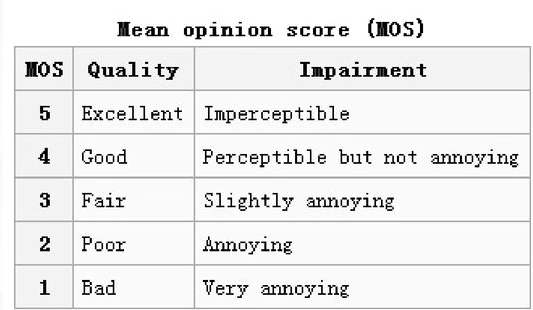
\includegraphics[scale = 0.5]{MOS}
\end{figure}

主观测试可分为3种:1.质量测试。观察者应评定图像的质量等级;2.损伤测试。观察者要评审出图像的损伤程度;3.比较测试。观察者对一幅给定图像和另一幅或几幅图像做出质量比较。
\begin{figure}[h]
	\centering
	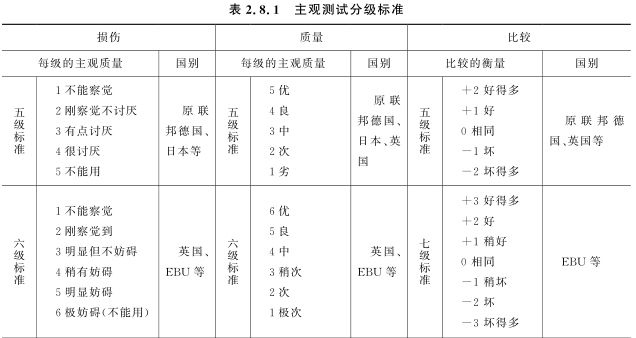
\includegraphics[scale = 0.7]{4}
\end{figure}
\subsubsection{客观评价指标}

客观评价方法:1.ITU-R视频质量专家组(VQEG,Video Quality Expert Group)规定的计算像素平均误差的客观质量评价方法。2.考虑人眼视觉特性的计算结构相似度的客观质量评价方法。

1.基于像素误差的评价

对于数字图像,设f(m,n)为原参考图像,$\hat{f}$(m,n)为其失真图像,尺度皆为MxN,定义失真图像的均方误差值(MSE,Mean Square Error)为
$$MSE = \frac{1}{MN}\sum_{n=1}^{N}\sum_{m=1}^{M}[f(m,n)-\hat{f}(m,n)]^2$$
在MSE的基础上定义失真图像的峰值信噪比(PSNR,Peak Signal Noise Ratio)为
$$PSNR = 10\cdot lg \frac{A^2}{MSE}(db)$$
其中A为原图像的最大灰度值。

所具有的局限性:1.需要原始图像进行对比。2.不一定能够准确地反映主观图像质量值,相同的PSNR值并不一定表示其主观质量一样,主观上好的图像不一定PSNR值高。

2.基于结构相似度的评价

基于结构相似度(SSIM,Structure Similarity)图像质量评价方法认为,相对于亮度和对比度信息,人类视觉系统对图像中的结构信息高度敏感,具有自动从视觉感知中提取结构信息的能力,因此结构信息量的变化能够反映一幅图像视觉感知失真的程度。而且,从图像形成的角度上来看,结构信息反映了场景中物体的结构,它基本独立于图像的亮度和对比度,亮度或对比度的改变对图像结构信息影响不大。

SSIM的比较对象为两幅灰度图像X和Y,其中一幅为参考图像,另一幅为其失真图像。设x为图像X的像素,y为图像Y的像素,两者的总像素为N,l(X,Y)为它们的亮度比较式,c(X,Y)是对比度比较式,s(X,Y)是结构比较式,定义如下:
$$l(X,Y)=\frac{2\mu_X\mu_Y+c_1}{\mu_X^2+\mu_Y^2+c_1}$$
$$c(X,Y)=\frac{2\sigma_X\sigma_Y+c_2}{\sigma_X^2+\sigma_Y^2+c_2}$$
$$s(X,Y)=\frac{\sigma_{XY}+c_3}{\sigma_X\sigma_Y+c_3}$$
将上述的各式组合起来成为图像X和Y的SSIM指数。
$$SSIM(X,Y)=[l(X,Y)]^{\alpha}[c(X,Y)]^{\beta}[s(X,Y)]^{\gamma}$$
为了简化表达,设定$\alpha =\beta = \gamma = 1$,且$c_3=\frac{c_2}{2}$,则SSIM指数为:
$$SSIM(X,Y)=\frac{(2\mu_X\mu_Y+c_1)(2\sigma_{XY}+c_2)}{(\mu_X^2+\mu_Y^2+c_1)(\sigma_X^2+\sigma_Y^2+c_2)}$$

由于图像统计特征通常是非全局平稳的,对整幅图像计算SSIM指数不如局部分块的效果好。例如,把图像分成不重叠的$8\times8$的小块,分块计算它们的SSIM值,整幅图像的SSIM值由各块的测量值加权平均得到,也可以简单平均得到。
$$SSIM(X,Y)=\frac{1}{M}\sum_{j=1}^{M}SSIM(bx_j,by_j)$$
其中X和Y分别是参考图像和失真图像,$bx_j$和$by_j$分别为X,Y对应位置的第j个小块,M是图像的小块个数。

目前相对成熟的是对黑白图像质量的定量评价,而对彩色图像在实用中往往将彩色图像的各个彩色分量作为灰度图像来评价,所有分量图像质量的平均就是该彩色图像的质量评分。

\subsection{其他评价方法}
\subsubsection{基于感兴趣区域的评价}
在进行PSNR计算时,对人眼感兴趣区域的像素给予更大的权值,加重ROI(Region of Interest)对图像质量结果的影响。这种方法较通常对整幅图像的所有像素平等对待更为合理(符合人眼的视觉心理要求)。
\subsubsection{联合视听评价}
一般情况下,我们在观看视频时都伴有声音,此时对图像质量的评价往往需要联合考虑音频和视频质量之间的相互作用。有以下结论:1.音频质量和视频质量共同贡献于整体的视听质量。2.一般情况下总体质量中视频质量占优势,而在音频和视频编码比特率都很低的情况下,或者视频质量已经大于某个门限值时,音频质量比视频质量更重要,并且随着音频质量的降低在总体质量中的影响逐渐增加。3.某些应用场景下,音频比视频内容更为重要。4.视听质量还会被其他因素影响,包括运动信息和视频内容的复杂性。
\subsubsection{无参考图像的评价}
在实际应用中,经常得不到参考图像或者获得参考图像的代价太大,因而要求评价方法降低对参考图像的依赖程度。经验表明,有时并不需要参考图像也能够对图像质量做出合理的评价,只要观测者在进行评价时抓住反映图像质量最本质的特征,如平滑程度,细节可分辨程度,彩色鲜艳程度。目前较为成熟的方法有面向特定失真和面向非特定失真的两类评价方法。特定失真有模糊失真,噪声干扰,块效应失真,JPEG压缩失真等。
\subsubsection{基于机器学习的评价}
机器学习作为一种数据驱动型的智能化信号处理工具已经开始应用于图像质量评价邻域,出现了多种接近主观评价的图像质量评价算法。如基于支持向量机(SVM,Support Vector Machine)分类器的训练,通过分析小波系数来提取图像中的特征。
\section{数字图像基础}
\subsection{人眼视觉特性}
\subsubsection{亮度适应性}
数字图像作为离散的灰度值来显示,所以眼睛对不同亮度级别之间的辨别能力在显示图像处理结果中是一个重要的考虑因素。
人的视觉系统的亮度适应范围从暗视觉极限到强光视觉极限之间的范围有$10^6$量级。但人的视觉系统在同一时刻所能够区分的亮度的具体范围比总的适应范围要小得多,一般仅在几十级亮度左右。

人眼从较亮的场所到较暗的场所时,很难马上看清东西;从较暗的场所到较亮的场所时,也很难看清东西。一般把眼睛的状态适应明暗条件的变化过程叫作亮度适应。从亮到暗的变化叫做暗适应;从暗到亮的变化叫作亮适应。一般亮适应时间较短,为暗适应时间较长。

在一定范围内与人眼所得到的照度基本成对数关系,即随着照度的线性增加所感知的亮度以对数关系缓慢增加(对暗光时亮度的增加比亮光时亮度的增加更敏感)。

第一种现象是马赫带效应,即视觉系统有趋向于过高或过低估计不同高度区域边界值的现象。尽管各条带内部的亮度是恒定的,但人们实际中总会观察到带有强烈边缘效应的灰度模式,即在条带的边界区域,靠更亮的一侧显得比较黑,而靠更暗的一侧显得比较白。
\begin{figure}[H]
	\centering
	
\includegraphics[scale=0.5]{5}
\end{figure}

第二种现象是同时对比度,即一个区域的感知亮度并不只是取决于其灰度。此现象基于人眼对某个区域感觉到的亮度并不仅仅依赖于区域本身的亮度,也同时受到图像背景的影响。
\begin{figure}[h]
	\centering
	
\includegraphics[scale=0.5]{6}
\end{figure}
\subsubsection{视错觉}
常见的视错觉几大类型:

(1)形状和尺寸错觉。
\begin{figure}[H]
	\centering
	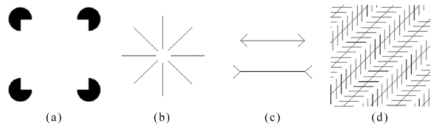
\includegraphics[scale=0.5]{7}
\end{figure}

(2)前景和背景错觉
\begin{figure}[H]
	\centering
	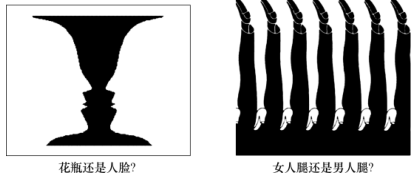
\includegraphics[scale=0.5]{8}
\end{figure}
图形在视网膜上是固定不动的,但你对它的感觉却是在两种可能图形中动摇,同时感觉到两种有意义的图形是很困难的。

(3)凹凸错觉
\begin{figure}[H]
	\centering
	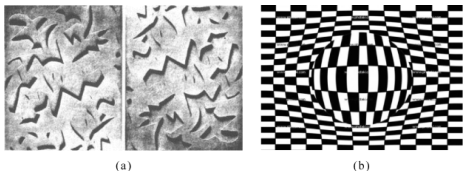
\includegraphics[scale=0.5]{9}
\end{figure}
在图像上由于明暗和阴影的影响,我们会得到凸出或凹入的错觉。同一张图像中的物体明亮部分在上方,阴影部分在下方,看上去这个物体是凸出的,把这张图像上下倒置过来,便会得到凹入的知觉。

(4)动静错觉
\begin{figure}[H]
	\centering
	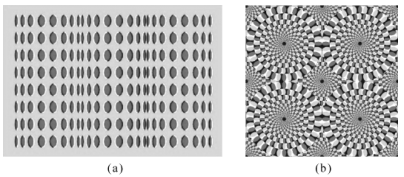
\includegraphics[scale=0.5]{10}
\end{figure}
\subsubsection{视觉惰性}
视觉惰性描述了主观亮度与光作用时间的关系。人眼主观亮度感觉的变化滞后于实际亮度变化,并且当光线消失后,人眼的亮度感觉不会随着物体亮度的消失而立即消失,而有一个过渡时间,这就是视觉惰性。

视觉暂留时间为0.05~0.2s,视觉暂留过渡时间内,亮度感觉按指数规律逐渐减少。

当人眼受周期性的光脉冲照射时,如果光脉冲频率不高,则会产生一明一暗的闪烁感觉。如果将光脉冲频率提高到某一定值以上,由于视觉惰性,眼睛便感觉不到闪烁,感到的是一种均匀的连续的光刺激。刚好不引起闪烁感觉的最低频率,称为临界闪烁频率,它主要与光脉冲的亮度有关。利用这一特性,每秒25帧的画面可形成连续活动图像的感觉。

在帧频率高于临界闪烁频率时,主观感觉亮度为显示亮度的平均值。隔行扫描就是利用这一特性克服闪烁现象的,同时还可以降低行扫描的频率,使得传输频带得以压缩。
\subsection{图像感知与获取}
我们感兴趣的大多数图像,都是由照射源和形成图像的场景元素对光能的反射或吸收产生的。照射源可来自非传统光源(如超声波),甚至来自计算机产生的照射模式。

在某些应用中,反射的能量或透射的能量被聚集到一个光转换器中,光转换器把能量转换为可见光。将照射能量转换为数字图像的三种主要传感器配置:单个成像传感器,条带传感器,阵列传感器。原理:组合输入电能和传感器对正被检测能量类型的响应,将入射能量转换为电压。输出电压波形是传感器的响应,将传感器响应数字化,得到一个数字量。

\subsection{连续图像函数}
图像是通常意义下光辐射和场景物体反射的共同结果,用辐射的强度,即图像的亮度表示光强度的空间分布,形成空间坐标(x,y,z)的函数,如$f(x,y,z)$。

一幅彩色图像,各点值还应反应出色彩变化,用$f(x,y,z,\lambda)$表示,$\lambda$为波长。

一幅活动的彩色图像,还应是时间t的函数,可以表示为连续的多维函数。
$$I = f(x,y,z,\lambda,t)$$
其中,x,y,z表示空间某点的坐标,t为时间轴,$\lambda$为光的波长。

在现实世界中,由于I表示的是物体反射,投射或辐射的光能量,所以I为一个非负,连续的有限函数,即$0\le I\le I_{MAX}$。其中$I_MAX$表示I的最大亮度值,一般I=0表示黑色,负的亮度值一般 没有实际的物理意义。 

人眼所能够感知的景物一般必须是连续的,以此不管中间过程如何用数字的方法进行处理,最终提交给眼睛的图片必须是连续的,即连续图像或模拟图像。
\subsection{常见图像种类}

常见的图像处理是在以计算机为中心的,包括多种输入,输出,储存,传输及显示设备在内的数字图像处理系统上进行的。目前常用的图像分为两类:1.连续(或模拟)图像,如从传统照相机,摄像机获得的图像;2.直接获得数字图像,如数码相机,数字摄像机等。

\begin{figure}[h]
	\centering
	\rotatebox[origin=c]{90}{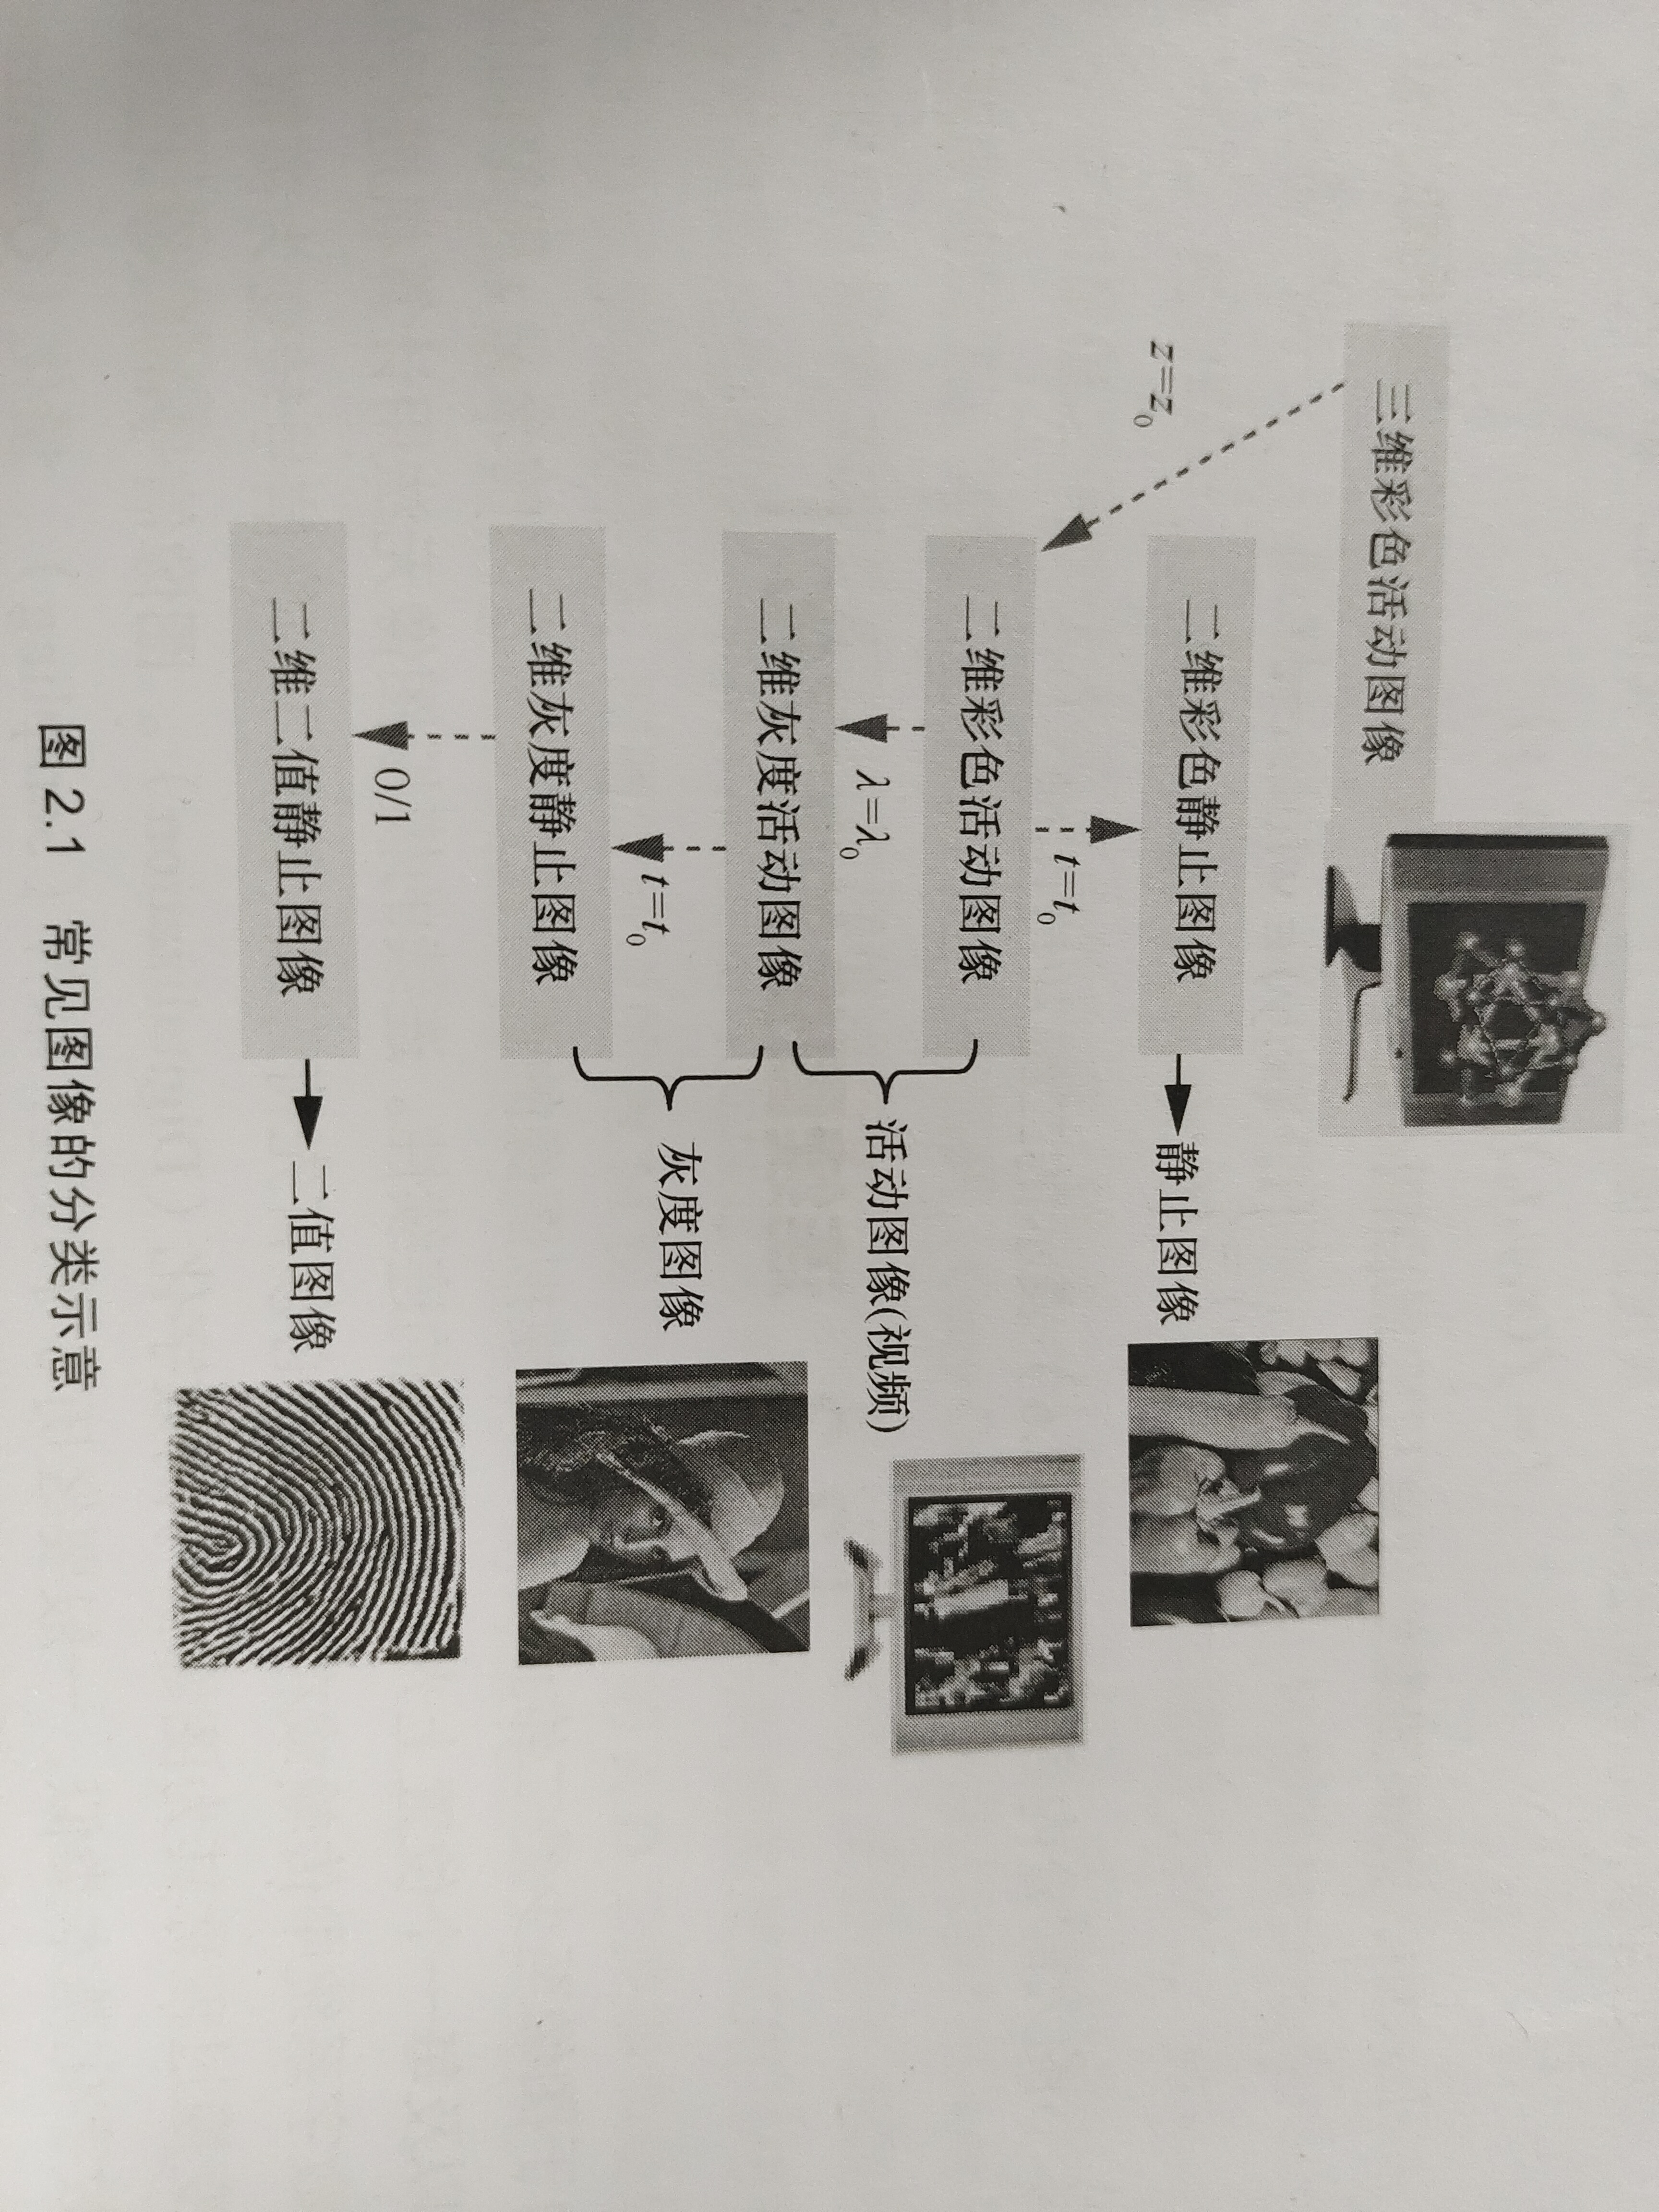
\includegraphics[scale=0.06]{1}}
\end{figure}
一个三维,彩色,活动的图像:
$$I = f(x,y,z,\lambda,t)$$

取$z=z_0$时,或不考虑深度信息时,则表示为一个二维,彩色,活动的图像:

$$I = f(x,y,z_0,\lambda,t)\qquad \text{或} \qquad I = f(x,y,\lambda,t)$$

取$t=t_0$时,图像内容不随时间变化,则表示为二维,静止的彩色图像:
$$I = f(x,y,\lambda,t_0) \qquad \text{或} \qquad I = f(x,y,\lambda)$$

可根据红黄蓝(RGB,Red Green Blue)三基色原理,将$I$分解为3个基色分量图像$I_R,I_G,I_B$:
$$
\left\{\begin{matrix}
	I_R = f_R(x,y,\lambda_R) \\ 
	I_G = f_G(x,y,\lambda_G) \\
	I_B = f_B(x,y,\lambda_B) \\
\end{matrix}\right.
$$
其中,$\lambda_R,\lambda_G,\lambda_B$为3个基色波长。

取$\lambda = \lambda_0$,当$\lambda$取为定值时,表示单色图像,则表示为二维,活动,灰度(单色)图像:
$$I = f(x,y,\lambda_0,t)\qquad \text{或} \qquad I = f(x,y,t)$$

取$t=t_0$,或者图像内容不随时间变化,则表示二维,静止,灰度图像,简称灰度图像:
$$I = f(x,y,t_0)\qquad \text{或} \qquad I = f(x,y)$$

在上式中,如果灰度只取黑白两个值,就形成了二值图像:
$$I = f(x,y) = \left\{\begin{matrix}
	1, \qquad (x,y)\in white\ erea \\ 
	0, \qquad (x,y)\in black\ erea \\
\end{matrix}\right.$$
\subsection{连续图像的数字化}
图像信号的数字化过程和其他模拟信号数字化过程基本相似,一般要经历3个过程:取样(Sampling),量化(Quantization)和编码(Coding)。

(1)取样(二维奈奎斯特取样定理)

图像$f(x,y)$的定义域在二维空间(x-y平面)上的坐标进行离散化过程称为取样或抽样。被选取的点称为取样点,抽样点或样点,这些取样点也称为像素(pixel)。在取样点上的函数值称为取样值,抽样值或样值。取样就是在定义域空间(图像)上用有限的取样点来代替连续无限的坐标值。一般情况下,水平方向的采样间隔和垂直方向的采样间隔相同。

具体做法是:先沿垂直方向按一定间隔从上到下按顺序地沿水平方向直线扫描,取出各水平线上灰度值的一维扫描,再对一维扫描线信号按一定间隔采样得到离散信号,即先沿垂直方向采样,再沿水平方向采样。

(2)量化(操作完后一定失真)

对每个取样点函数值(灰度)的离散化过程为量化。即用有限个数值来代替连续无限多的灰度值。把采样后所得到的各像素的灰度值从模拟量到离散量的转换称为图像灰度的量化。量化两大类,1.将每个样值独立进行量化的标准量化(Scaling Quantization),还可继续分为均匀量化(将样点灰度值等间隔分档,通常采用的是编码中的PCM编码),非均匀量化(不等间隔分档)。2.将若干样值联合起来作为一个矢量来量化的矢量量化(Vector Quantization)。

(3)编码

将经过量化后的离散灰度值用适当的二进制(或其他进制)数来表示。有不同的编码方法,只要保证量值和号码之间的对应关系即可。常见的编码方法有:PCA(Pulse Code Modulation)脉冲编码调制,格雷码(Gray Code)和循环码(Cyclic Code)
\subsubsection{数字图像表示}
令$f(s,t)$表示一个有两个连续变量$s$和$t$的连续图像函数。通过取样和量化,我们可把函数转换为数字图像。假设这幅连续图像取样为一幅数字图像$f(x,y)$,该图像包含有$M$行和$N$列,其中$(x,y)$是离散坐标。由图像的坐标张成的实平面部分称为空间域,x和y称为空间变量或空间坐标。

我们将图像的左上角定义为原点:许多图像显示器扫描图像时都从左上角开始向右移动,每次扫描一行。矩阵的第一个元素按照惯例应在矩阵的左上角,将$f(x,y)$的原点选择为左上角数学上是可行的。原点为$(0,0)$,范围在$(M-1,N-1)$的$M\times N$数字图像的中心,由$M$和$N$除以2后四舍五入为最接近的整数得到。

图像数字化要求对M值,N值和离散灰度级数L进行判定。对于M和N,除必须取整数外,并无其他限制。然而出于存储和量化硬件的考虑,灰度级数通常取为2的整数次幂。灰度跨越的值域称为动态范围,通常将图像系统的动态范围定义为系统中最大可度量灰度与最小可检测灰度之比。通常,上限取决于饱和度,下限取决于噪声,但噪声也会出现在较亮的灰度中。

图像对比度:一幅图像中最高和最低灰度级间的灰度差。反差比是这两个量的比率。一幅图像中的可观测像素数量具有高动态范围时,我们称该图像具有高对比度。相反,具有低动态范围的图像看起来通常很灰暗。
\subsubsection{图像的数学模型}
在计算机中,图像被分割成一个一个的像素,各像素的灰度值用整数表示。一幅$M\times N$个像素的数字图像,其像素灰度值可以用M行N列的矩阵$f(i,j)$表示:
$$f(i,j) = \begin{pmatrix}
	f_{11}& f_{12} & \cdots & f_{1N}\\
	f_{21}& f_{22} & \cdots & f_{2N}\\
	\vdots & \vdots & & \vdots\\
	f_{M1}& f_{M2} & \cdots & f_{MN}\\
\end{pmatrix}$$

在计算机中把数字图像表示为矩阵后,就可以用矩阵理论和其他一些数学方法来对数字图像进行分析和处理了。
\subsubsection{二维图像频谱}

二维图像信号的频谱实际上就是图像函数的傅里叶变换(Fourier Transform)频域系数。

一维傅里叶变换,对于一维有界连续信号$f(x)$,其傅里叶变换将其变换到频率域中:
$$F(f) = \frac{1}{\sqrt{2\pi}}\int_{-\infty}^{\infty}f(x)e^{-j2\pi f(x)}dx$$
频率函数$F(f)$为$f(x)$的频谱,表示$f(x)$在频谱率的分布。

二维连续图像信号$f(x,y)$的傅里叶变换$F(u,v)$:
$$F(u,v) = \frac{1}{\sqrt{2\pi}}\int_{-\infty}^{\infty}\int_{-\infty}^{\infty}f(x,y)e^{-j2\pi (ux+vy)}dxdy$$
它表明了图像的空间频率成分,即在二维频率的分布情况其中,u表示水平方向的频率成分,v表示垂直方向的频率成分。

对于要处理的实际二维图像,其傅里叶变换一般在频率域上是有界的,即信号频率的有用成分总是落在一定的频率域范围之内。图像的频谱大多局限在一定的范围内,过高的频率分量没有多大的实际意义。
\subsubsection{取样函数阵列}
由于冲激函数独特的性能,它对信号处理系统进行测量或提取。从而获得信号或系统的特性参数。

一维冲激函数$\delta(x)$又称Drac函数,是连续域的一种广义函数,其定义为:

$$\delta(x)  = \left\{\begin{matrix}
	\infty, &x = 0 \\ 0, &\text{其他}
\end{matrix}\right. \text{,且满足} \int_{-\infty}^{\infty}\delta(x)dx = 1$$

二维冲激函数定义为二维Drac函数$\delta(x,y)$为:

$$\delta(x,y)  = \left\{\begin{matrix}
	\infty, &x = y = 0 \\ 0, &\text{其他}
\end{matrix}\right. \text{,且满足} \int_{-\infty}^{\infty}\int_{-\infty}^{\infty}\delta(x,y)dxdy = 1$$

由无穷多个经过规则位移的二维Drac函数可以组成一个空间域上的二维Drac函数无穷阵列$s(x,y)$,表达式为:
$$s(x,y) = \sum_{m=-\infty}^{\infty}\sum_{n=-\infty}^{\infty}\delta(x - m\Delta x,y - n\Delta y)$$

其傅里叶变换是频域中$\delta$函数的无穷阵列$S(u,v)$,表达式为:
$$S(u,v) = \frac{1}{\Delta x\Delta y}\sum_{i=-\infty}^{\infty}\sum_{j=-\infty}^{\infty}\delta(u - \frac{i}{\Delta x},v - \frac{j}{\Delta y})$$

二维Drac函数$\delta(x,y)$具有以下几个性质:

\noindent(1)抽样性质(乘积)$$f(x,y)\delta(x-\alpha,y-\beta)=f(\alpha,\beta)\delta(x-\alpha,y-\beta)$$
\noindent(2)筛选性质(卷积)$$\sum_{-\infty}^{\infty}\sum_{-\infty}^{\infty}f(x,y)\delta(x-\alpha,y-\beta)dxdy=f(\alpha,\beta)$$
\noindent(3)偶函数和可分离$$\delta(-x,-y)=\delta(x,y)=\delta(x)\cdot\delta(y)$$
\noindent(4)卷积$$\delta(x-x_1,y-y_1)\ast\delta(x-x_2,y-y_2)=\delta[x-(x_1+x_2),y-(y_1+y_2)]$$
\noindent(5)尺度变化$$\delta(ax,by)=\frac{1}{\left|a\right |\cdot \left|b\right |}\cdot\delta(x,y)\text{,\quad a$\cdot$ b$\neq$ 0 }$$
\noindent(6)傅里叶变换

\noindent 对于任意常数k,$k\delta(x,y)$的傅里叶变换为k。
\subsubsection{连续图像的取样}
连续图像的取样就是图像空间位置的离散处理。

1.二维取样定理

奈奎斯特取样定理:一维带限模拟信号的数字化取样过程中,考虑的是信号频带宽度和取样间隔之间的关系。

二维取样定理:一连续图像在水平方向的截止频率为$U_m$,在垂直方向上的截止频率为$V_m$,只有在水平方向的空间取样频率$U_0\geqslant2U_m$,垂直方向的空间取样频率$V_0\geqslant2V_m$,即取样点的水平距离$\Delta x\leqslant\frac{1}{2U_m}$,垂直间隔$\Delta y \leqslant\frac{1}{2V_m}$,图像可被精确地恢复。

2.取样图像的重建

在满足取样定理的条件下,各周期延拓的频谱区域互不重叠。重建原图像的简单方法是用一个中心位于原点的理想二维方形滤波器完整地将频谱中地各个高次谐波滤除,利用剩下地基波分量就可以恢复原始图像。

\subsubsection{取样值的量化}
经过取样的图像,只是在空间上被离散成为像素的阵列。但每个样本灰度还是一个有无穷多取值的连续变化量,将有无穷多个值的连续量转化为有限数量的离散量的过程称为量化。

在两个判决电平将连续的灰度范围分为8个等份,形成8个量化间隔(区域)。在两个判决电平之间的所有灰度值用一个量化值(称为量化器输出的量化电平)来表示。

量化既然是以有限个离散值近似表示无限多个连续量,就一定会产生误差。当量化层数减少到一定程度时,量化值与连续值之间的差值(量化误差)变得很显著,引起严重的图像失真,尤其在原先亮度值缓慢变化的区域会引起生硬的“伪轮廓”。

图像量化的基本要求是在量化噪声对图像质量影响一定的前提下用最少的量化层进行量化。

通常对取样值进行等间隔的均匀量化,量化层数K取为$2^n$。每个量化层的量化电平可以采用n bit自然二进制数表示,形成PCM编码。量化分层越多,量化误差越小,但编码是占用比特数就越多。

\subsubsection{量化值的编码}
模拟图像在经过取样,量化和编码后形成二进制比特表示,就完成了图像的数字化。

数字化的图像是指用二进制(或多进制)的符号按一定的顺序表示每个像素点的量值。

图像的采样值在量化以后形成有限数量的量化值,量化值是一个标号,每个标号表示该量化值属于某个量化区间。量化的本质就是给一组量化区间发放标号,为了适应二进制的应用,将十进制标号编上一个二进制的码。

最简单的编码方法是二进制PCM编码:等长度的自然二进制码按大小顺序排列,需要编码的量化值也按大小顺序进行排列,然后进行一一对应的编码。

\subsubsection{量化失真}

在不考虑取样密度不足带来的混叠失真(Aliasing Distortion),编码和量化值形成一一对应的关系,那么在图像数字化的过程中,只有量化会给图像带来失真。

一帧图像可以描述成$N\times N$的m位像素,其中N是点的数目,m表示亮度值的级数。m位(bit)给出$2^m$个值,范围从0到$2^m-1$。如下图所示,m值越小,则有效的亮度级也越小,从而减少图像中的有效对比度。

选择8位像素的优点:1.8位能够包括模拟摄像机的有效范围。2.方便把像素值存储成字节(byte),而且8位A/D转换器比高分辨率更便宜。

对于一般的应用,如数字化图像,数码照相,电视广播,视频通信等,经常采用8bit量化,已基本满足要求。对于某些应用,如高质量的静止图像,遥感图像,医学图像处理等,需要10bit,12bit或更高精度的编码比特。
\begin{figure}[H]
	%\centering
	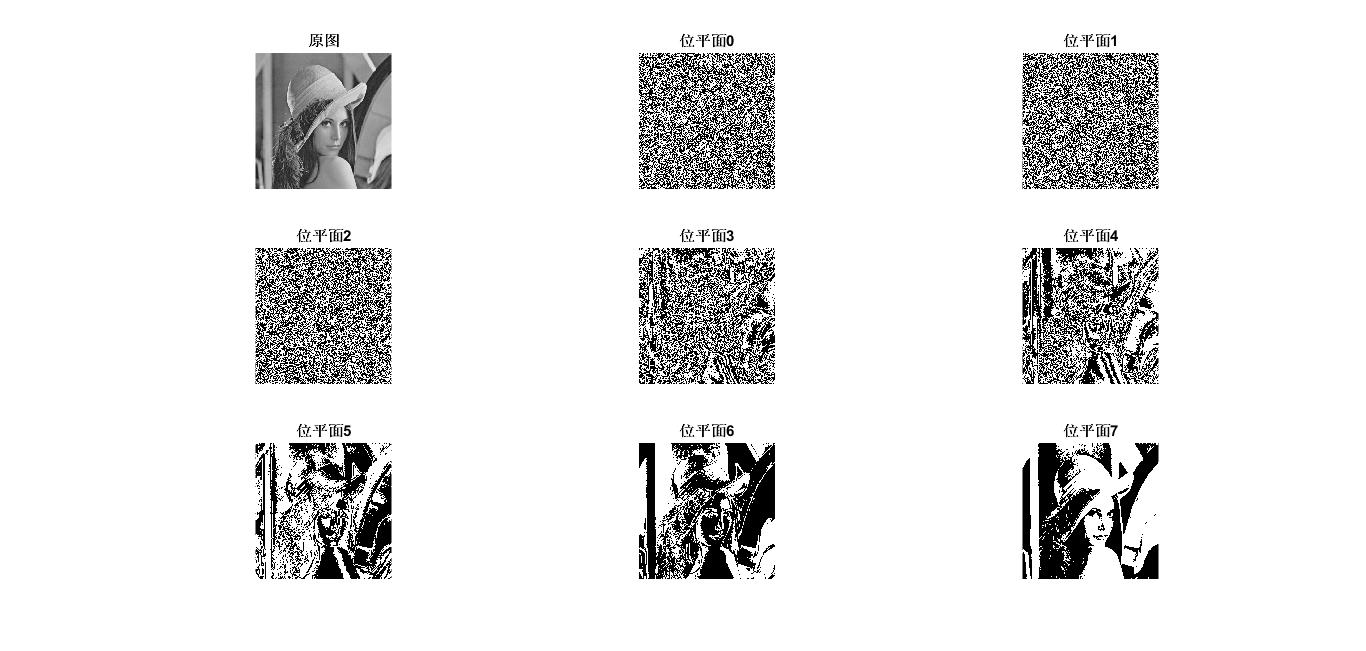
\includegraphics[scale = 0.4]{11}
\end{figure}
\subsubsection{图像内插}
内插通常在图像放大,缩小,旋转和几何校正等任务中使用。内插是用已知数据来估计未知位置的值的过程。

\begin{figure}[h]
	\centering
	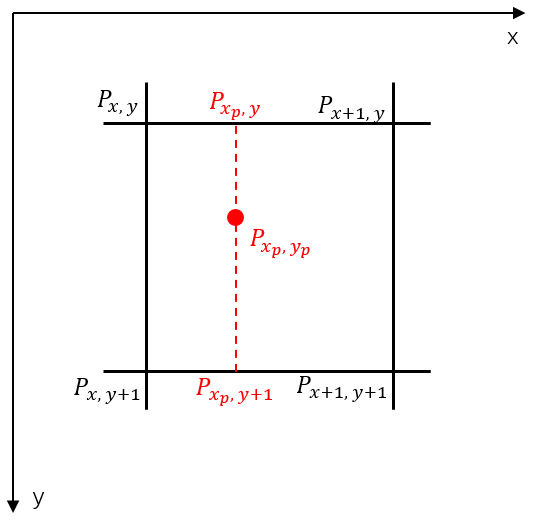
\includegraphics[scale=0.4]{52}
\end{figure}
\textbf{最邻近插值}:将距离$P_{x_p,y_p}$最近的已知点的像素值$P_{x,y}$直接赋值给$P_{x_p,y_p}$。假设大小为$500\times 500$像素的一幅图像要放大1.5倍。创建一个大小为$750\times 750$像素的假想网格,网格的像素间隔完全与原图像的像素间隔相同,然后收缩网格,使它完全与原图像重叠。对于没赋值的像素值取原图像中最接近的像素。

这种插值方法计算量非常小,且非常简单,不会产生出任何新的像素值,所有插值出来的像素值必然来自于原图的某个像素。但是视觉效果往往不是太好,特别是图像内的一些线条和边缘(edge)会出现明显的锯齿效应。

\textbf{双线性插值}:它使用了4个最近邻的灰度来计算给定位置的灰度。在图像双线性插值中,有时候我们需要知道一个位置的像素值,而这个位置恰好不在像素点上(对应坐标一般来说不是整数,而非整数的坐标是无法在图像这种离散数据上使用的),因此,要用该位置周围的4个像素点的值来估计该点的值。

内插时可以使用更多的邻点,并且存在使用样条和小波的复杂技术,采用这些技术可以得到更好的结果。
\subsubsection{像素间的关系}
令$V$是用于定义邻接的灰度值集合。考虑三种类型的邻接:

一.4邻接。q在集合$N_4(p)$中时,值在$V$中的两个像素$p$和$q$是4邻接的。
\begin{figure}[h]
	\centering
	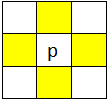
\includegraphics[scale=0.4]{53}
\end{figure}

二.8邻接。q在集合$N_8(p)$中时,值在$V$中的两个像素$p$和$q$是8邻接的。
\begin{figure}[h]
	\centering
	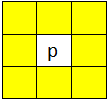
\includegraphics[scale=0.4]{54}
\end{figure}

三.m邻接(混合邻接)。 p和q是4邻接的或者p和q是8邻接且p的四邻域和q的四邻域的交集中没有V中的元素。

\begin{wrapfigure}{r}{7.7cm}
	\centering
	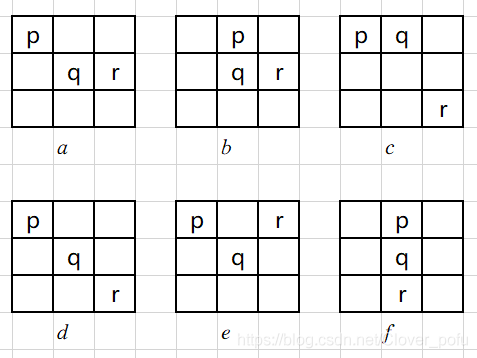
\includegraphics[width=0.33\textheight]{55}
\end{wrapfigure}

图(a)中,p和q是m邻接、8邻接的。q和r是m邻接、4邻接的。p和r不邻接。

图(b)中,p和q是m邻接、4邻接的。q和r是m邻接、4邻接的。p和r是8邻接、但不是m邻接的(因为p和r的4邻域交集中,有个q是属于V的)。

图(c )中,p和q是m邻接、4邻接的。r没有和p或q邻接。

图(d)中,p和q是m邻接、8邻接的。q和r是m邻接、8邻接的。p和r不邻接。

图(e)中,p和q是m邻接、8邻接的。q和r是m邻接、8邻接的。p和r不邻接。

图(f)中,p和q是m邻接、4邻接的。q和r是m邻接、4邻接的。p和r不邻接。
\subsection{混叠和亚取样}
\subsubsection{混叠效应}
频谱的混叠(Aliasing):取样频率小于奈奎斯特取样频率,或图像为非限带信号,取样图像频率的各次谐波就会发生重叠。

混叠失真:对于已发生混叠的频谱,在图像的恢复中都将会引入一定的失真。实际工程中,需要的是尽可能地将混叠失真控制在一个允许地范围内。

在实际图像处理中,取样后图像信号的频谱混叠是不可避免的,因为图像信号并非真正的邻域限带信号。任何空域(或时域)范围有限的信号,其频域范围必为无限的。

\subsubsection{反混叠失真}
减少混叠失真地方法是提高取样频率,但实际情况取样频率无法随意提高。一般可采用反混叠滤波地方法来减少混叠效应。

取样频率地混叠往往发生在频谱地高端,因此较为方便地方法是用一低通滤波器将引起混叠地高频分量予以滤除,形成符合取样定理地限带信号,再进行取样。

一般会产生两种失真,一种是混叠失真,一种是高频失真,权衡两者利弊的结果,宁可损失一点高频分量,也不能容忍由邻近频谱的叠加而形成新频率分量的混叠失真。

反混叠滤波的实现方法:1.模拟滤波,先对模拟信号进行低通滤波,然后对滤波后的图像进行取样,效果还可以,但是实现起来不灵活。2.数字滤波,先用足够高的取样频率对图像进行数字化,再对数字化后的图像进行数字低通滤波,最后对滤波后的数字图像按照要求用较低的频率进行再取样。数字域实现各种滤波方便。

\begin{figure}[h]
	\centering
	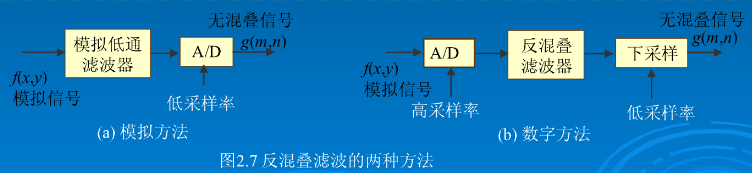
\includegraphics[scale = 0.5]{12}
\end{figure}
\subsubsection{亚取样}
亚取样(Sub-sampling):采用低于取样频率的脉冲来取样频率来取样来减少图像数据量最直接,简单的方法。

菱形亚取样(Diamond Subsampling)可以在亚取样的场合大大减少混叠失真。经过大量的统计分析,常见自然图像的频谱主要分布在二维频谱中以原点为中心,4个顶点在u,v轴上的一个菱形范围内,反应在频谱中就是水平和垂直方向的高频分量比其他方向丰富,频谱的有效区域呈现为菱形。

\begin{figure}[h]
	\centering
	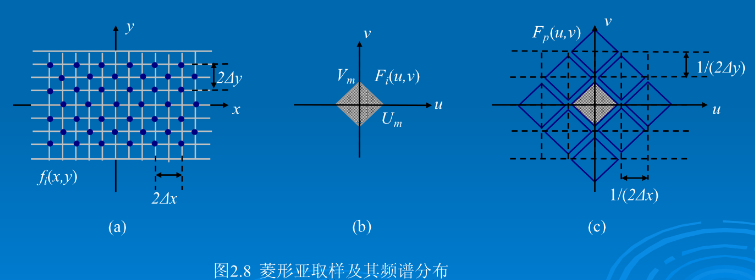
\includegraphics[scale = 0.5]{13}
\end{figure}

\subsubsection{实际取样脉冲影响}
图像的实际取样过程中,既要考虑混叠失真,也要考虑取样脉冲的影响。

如果实际取样脉冲足够窄时可予以忽略。如果要消除实际取样脉冲对取样的影响,在很多情况下可以用和取样脉冲特性相反的滤波加以校正。

滤波可以在连续域或离散域上进行,但是一般在离散域上更加方便。

\subsection{数字图像的分辨率}

图像的分辨率(Resolution)是表征图像质量的一个主要参数。数字图像采样和量化参数的选择直接影响图像的数据量,实际上也会影响人们的视觉效果和对图像的进一步处理。图像的分辨率是指图像所表示的场景中可以区分的最小差别,常见的分辨率:1.空间分辨率,用于表示图像对空间位置的区分能力。2.灰度(彩色)分辨率,用于表示图像对灰度深浅或彩色种类的区别能力。3.时间分辨率,用于表示对不同时间图像变化的区别能力。
\subsubsection{空间分辨率}
数字图像的空间分辨率可用单位面积的像素数来表示,而单位面积的像素数直接取决于采样频率或采样间隔。对于同一场景的同样尺寸的图像,空间分辨率越高意味着图像越清晰。为了计算方便,图像的尺寸常用2的整数幂来定义。不考虑图像压缩的情况下,空间分辨率的本质是描述同一场景花费的信息量(多少比特)

高分辨率的获得是有代价的:1.提高取样密度,增加了图像采集和数字化的复杂度;2.生成的高清晰度图像的数据量随着空间分辨率的加大而迅速增大。因此,我们在选择图像的空间分辨率需在图像质量和花费代价之中做出折中的选择。

对于显示分辨率,在显示中,往往无论什么分辨率的图像都是以同样的显示屏(或打印纸)几何尺寸来显示。1.待显示图像的分辨率高于显示器,则显示器会降低图像的分辨率,以适应显示要求,或只显示图像的一部分。2.图像和显示器的分辨率一致时,显示器可以真实的反映图像的分辨率。3.图像的分辨率低于显示分辨率,显示有两种处理方式:按照显示器的分辨率来显示图像,这时所显示图像的尺寸会变小;将像素放大成像素块使得更多的显示单元来参与显示。

另外空间分辨率和人眼的视距有关,同样的分辨率的图像,随着视距的增加其感觉分辨率会逐渐下降。因此,在讨论图像空间分辨率时不考虑人眼视距的影响,或者默认在同一视距下进行比较。
\subsubsection{灰度分辨率}
灰度分辨率和取样值的量化环节直接相关。讨论的灰度分辨率对彩色图像同样适用,彩色图像可以分解为多幅单色图像,每一幅单色图像都可当作一幅灰度图像来处理。

图像的灰度分辨率是指将像素的总体灰度范围划分为多个等级,等级数越多,灰度分辨率越高,意味着图像的深浅层次越丰富,在图像中所能够分辨的细节越多。因此在一般情况下,我们希望图像的灰度分辨率越高越好,一幅数字图像灰度分辨率可以简单地用像素地比特数来表示。

随着灰度分辨率逐渐减少,图像中发生灰度“合并”区域不断增加,细节地模糊,边缘生硬地现象逐渐严重。灰度级数通常是2的整数次幂,通常是8比特,在需要增强特定灰度范围的某些应用中,也使用16比特。使用32比特的灰度量化很少见。

在一般情况下,我们希望显示器地显示特性是线性地,可以忠实地反映图像地灰度等级差别,但实际上,显示器(CRT,LCD,LED)地显示特性往往是非线性的。为了获得准确的灰度显示,必须对输出的显示器的图像数据预先加以校正,已获得尽可能的线性灰度显示。

一般来说,当限定数字图像的大小时,为了得到质量较好的图像,可采用如下原则:1.对缓变的图像,应细量化,粗采样,以避免出现假轮廓。2.对细节丰富的图像,应细采样,粗量化,以避免模糊。

细节丰富的图像可能只需要较少的灰度级,对于人群图像固定的像素点数,这类图像的感觉质量与所用灰度级数基本无关。
\subsubsection{时间分辨率}
图像的时间分辨率是针对活动图像(如视频,电影,动画等)而言的,用于表示对不同时间图像变化的区别能力。

实践证明,每秒达到10幅以上,人眼就可以产生明显的连续感。图像随时间更改的速度,即每秒显示图像的幅数(帧数)越多越好,即时间分辨率越高,我们看到的运动越平滑,越连续。因此,我们往往用帧数(即每秒显示的图像幅数)来表示时间分辨率。帧数越高,时间分辨率越高,人的动态视觉感受也越好。

但是,随着时间分辨率逐渐增加,同一场景活动图像的数据量也急剧增加,对拍摄器件和显示器件的要求也越加苛刻。

人眼对快速运动场景要求有较高的时间分辨率,而此时人眼的空间分辨率有所下降;相反,对相对静止的场景,人眼对图像的空间分辨率要求较高,对时间分辨率要求则可以有所下降。
\subsubsection{综合考虑}
简单综合地考虑这几个分辨率地影响:

\noindent(1)考虑图像质量:作为高质量地图像,既具有较高地空间分辨率,又具有较高的灰度分辨率和时间分辨率(活动图像)

\noindent(2)考虑图像的数据量:对于一幅$M\times N$的空间分辨率的L bit的灰度分辨率的数字图像,其总的数据量为$D=M\times N\times L$(比特/图像)

\noindent(3)考虑人眼的视觉特性:在图像中具有大量细节和跳变的区域,图像的灰度等级可以适当的减少,但是空间分辨率却要求较高。在图像的平缓区域可以放宽对空间分辨率的要求,但要求很细的灰度等级。

\noindent(4)考虑不同的分辨率组合:如果在给定一幅图像总数据容量的情况下,可以选择不同的空间分辨率和灰度分辨率组合,如对图像中感兴趣区间分配高分辨率,对其他区域则可降低分辨率,以取得最好的主观图像质量。

\section{图像变换和分析}
在数字信号处理中,通常有两种方法:一是时间域(或空间域)分析法,二是频率域(或变换域)分析法。数字图像处理:一是空间域图像处理,在空间域对图像的像素进行各种运算,卷积是其中最重要的处理方法,二是频率域图像处理,将图像信号从空间域变换到频率域,在频率域对变换系数进行各种运算,采用反变换的方法将频率处理的结果变换到空间域,使我们可以从另一角度分析图像信号的特性。

常见的图像变换有:傅里叶变换,余弦变换,沃尔什变换,阿达马变换等。每种变换都存在自己的正交集函数集。图像数据的主分量分析(PCA)和奇异值分解(SVD)本质也是一种变换,只不过是它们的基函数集不是固定的,而是和数据本身有关。

\begin{figure}[H]
	\centering
	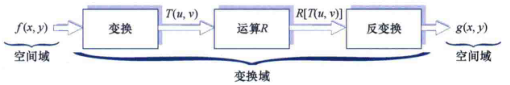
\includegraphics[scale=0.6]{57}
\end{figure}

\subsection{图像的代数运算}
图像的代数运算指两幅或多幅图像的加减乘除运算和一般的线性运算。
\subsubsection{图像的加运算}
设有两幅图像$A(x,y)$和$B(x,y)$,而$C(x,y)$为返回的图像,则图像的加运算的表达式为:$C(x,y) = A(x,y) + B(x,y)$。图像的加运算可生成图像叠加效果,得到各种图像合成的效果,也可以用于两张图像的衔接。
\subsubsection{图像的减运算}
设有两幅图像$A(x,y)$和$B(x,y)$,而$C(x,y)$为返回的图像,则图像的加运算的表达式为:$C(x,y) = A(x,y) - B(x,y)$。图像的减运算可提供图像间的差异信息,能用于混合图像的分离,指导动态检测,运动目标检测和跟踪,图像背景消除及目标识别等。
\subsubsection{图像乘运算}
设有两幅图像$A(x,y)$和$B(x,y)$,而$C(x,y)$为返回的图像,则图像的加运算的表达式为:$C(x,y) = A(x,y) \times B(x,y)$。图像的乘运算可用于图像的局部显示,实现掩膜处理,即屏蔽图像的某些部分。
\subsubsection{图像除运算}
设有两幅图像$A(x,y)$和$B(x,y)$,而$C(x,y)$为返回的图像,则图像的加运算的表达式为:$C(x,y) = A(x,y) \div B(x,y)$。图像的除运算可用于检测图像间的差别,主要是像素值的比率变化,因此也称为比率变换。
\subsection{图像的几何变换}
在实际生活中拍摄到的图像,如果画面过大或过小,都需要进行缩小或放大的调整。图像的几何变换是指图像处理中对图像进行平移,旋转,放大和缩小等简单变换以及变换中灰度内插处理等。几何变换可以改变图像中各物体之间的空间位置关系而不改变像素值。
\begin{figure}[H]
	\centering
	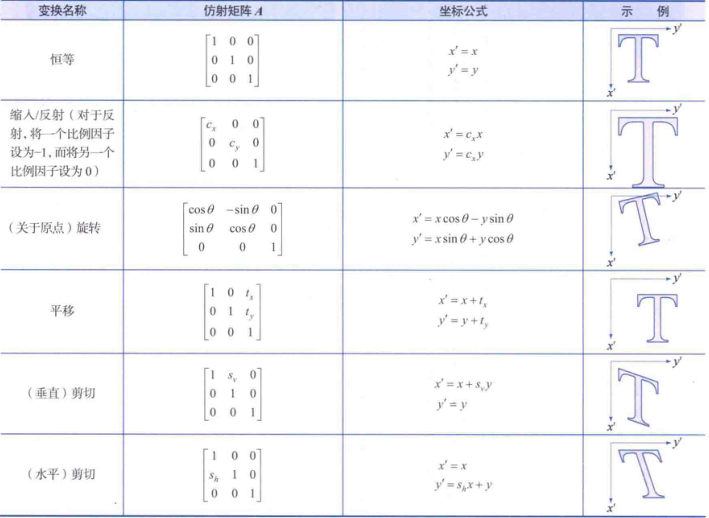
\includegraphics[scale=0.6]{56}
\end{figure}
\subsubsection{齐次坐标}
一幅数字图像可以用f(x,y)表示,其中(x,y)表示二维空间x,y中一个坐标点的位置,$f(x,y)$表示图像在点$(x,y)$处的像素值。

\begin{wrapfigure}{r}{4.9cm}
\centering
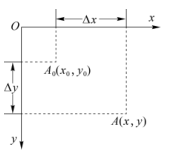
\includegraphics[width=0.23\textheight]{2}
\end{wrapfigure}
设点$A_0(x_0,y_0)$进行平移后移到$A(x,y)$, 其中x方向的平移量为$\Delta x$,y方向的平移量为$\Delta y$,则点$A(x,y)$的坐标可表示为:
$$\left\{\begin{matrix}
	x=x_0 + \Delta x\\ 
	y=y_0 + \Delta y
\end{matrix}\right.$$
用矩阵的形式则表示为:
$$\begin{pmatrix}x \\y\end{pmatrix}=\begin{pmatrix}x_0 \\y_0\end{pmatrix}+\begin{pmatrix}\Delta x \\ \Delta y\end{pmatrix}$$

几何变换一般形式可表示为:
$$\begin{pmatrix}x \\y\end{pmatrix}=T\begin{pmatrix}x_0 \\y_0\end{pmatrix}=\begin{pmatrix}a& b \\ c& d\end{pmatrix}\begin{pmatrix}x_0 \\ y_0\end{pmatrix}$$
但是由于矩阵T中没有引入平移常量,需要将矩阵T扩展为$2\times 3$变换矩阵。
$$\begin{pmatrix}x \\y\end{pmatrix}=T\begin{pmatrix}x_0 \\y_0\end{pmatrix}=\begin{pmatrix}1& 0 \\ 0& 1\end{pmatrix}\begin{pmatrix}x_0 \\ y_0\end{pmatrix} + \begin{pmatrix}\Delta x \\ \Delta y\end{pmatrix} = \begin{pmatrix}1 & 0 & \Delta x \\ 0 & 1 &\Delta y\end{pmatrix}\begin{pmatrix}x_0 \\ y_0 \\ 1\end{pmatrix}$$
为了变换运算时更加方便,一般将$2\times 3$阶变换矩阵T进一步扩充为$3\times 3$方阵。
$$T = \begin{pmatrix}1 & 0 & \Delta x \\ 0 & 1 &\Delta y\\ 0 & 0 & 1\end{pmatrix}$$

\subsubsection{平移变换}
用矩阵的形式则表示为:
$$\begin{pmatrix}x \\y \\1 \end{pmatrix}=\begin{pmatrix}1 & 0 & \Delta x \\ 0 & 1 &\Delta y\\ 0 & 0 & 1\end{pmatrix}\begin{pmatrix}x_0 \\ y_0 \\ 1\end{pmatrix}$$
平移后图像上的每一点都可以在原图像中找到其对应的点。对于不在原图像中的像素点,可以直接将它的像素值统一设置为0或者255,由此可对应灰度图像中的白色或者黑色。若图像平移后并没有被放大,说明移出的部分被截断,原图像中有像素点被移出显示区域。

\subsubsection{镜像变换}
\textbf{水平镜像}

水平镜像是将图像左半部分和右半部分以图像垂直中轴线为中心进行镜像对换操作。
\begin{wrapfigure}{r}{5cm}
	\centering
	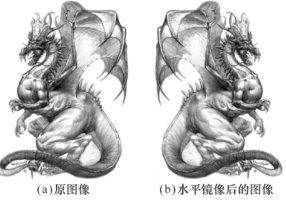
\includegraphics[width=0.23\textheight]{14}
\end{wrapfigure}

设点$A_0(x_0,y_0)$进行镜像后的对应点为$A(x,y)$,图像高度为$f_h$,宽度为$f_w$,源图像镜像操作的表达式:
$$\begin{pmatrix}x \\y \\1 \end{pmatrix}=\begin{pmatrix}-1 & 0 & f_w \\ 0 & 1 & 0\\ 0 & 0 & 1\end{pmatrix}\begin{pmatrix}x_0 \\ y_0 \\ 1\end{pmatrix}$$

更为普遍的规律,若$3\times 3$的图像矩阵为:
$$F = \begin{pmatrix}f_{11} & f_{12} & f_{13}\\f_{21} & f_{22} & f_{23} \\f_{31} & f_{32} & f_{33} \end{pmatrix}$$
经过水平镜面后的图像,行的排列顺序$i = 1,2,3$保持不变,将原来的列的排列顺序由$j=1,2,3$转换为$j=3,2,1$,即:
$$F = \begin{pmatrix}f_{13} & f_{12} & f_{11}\\f_{23} & f_{22} & f_{21} \\f_{33} & f_{32} & f_{31} \end{pmatrix}$$

\textbf{垂直镜像}

垂直镜像是将图像上半部分和下半部分以图像水平中轴线为中心进行镜像对换操作。
\begin{wrapfigure}{r}{5cm}
	\centering
	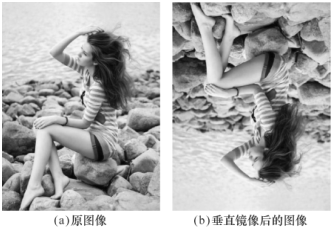
\includegraphics[width=0.23\textheight]{15}
\end{wrapfigure}

设点$A_0(x_0,y_0)$进行镜像后的对应点为$A(x,y)$,图像高度为$f_h$,宽度为$f_w$,源图像镜像操作的表达式:
$$\begin{pmatrix}x \\y \\1 \end{pmatrix}=\begin{pmatrix}1 & 0 & 0 \\ 0 & -1 & f_b\\ 0 & 0 & 1\end{pmatrix}\begin{pmatrix}x_0 \\ y_0 \\ 1\end{pmatrix}$$

若$3\times 3$的图像矩阵,经过垂直镜像后的图像,列的排列顺序$j=1,2,3$保持不变,将原来的行排列顺序由$i = 1,2,3$转换为$i = 3,2,1$即:
$$F = \begin{pmatrix}f_{31} & f_{32} & f_{33}\\f_{21} & f_{22} & f_{23} \\f_{11} & f_{12} & f_{13} \end{pmatrix}$$

\textbf{对角镜像}

对角镜像是将图像以图像水平中轴线和垂直中轴线的交点为中心进行镜像对换操作,也相当于将图像先进行水平镜像再进行垂直镜像,或将图像先进行垂直镜像再进行水平镜像。
\begin{wrapfigure}{r}{6.7cm}
	\centering
	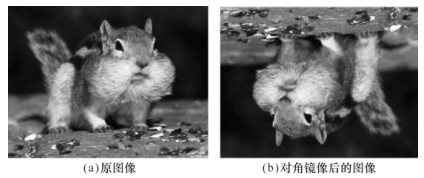
\includegraphics[width=0.32\textheight]{16}
\end{wrapfigure}

设点$A_0(x_0,y_0)$进行镜像后的对应点为$A(x,y)$,图像高度为$f_h$,宽度为$f_w$,源图像镜像操作的表达式:
$$\begin{pmatrix}x \\y \\1 \end{pmatrix}=\begin{pmatrix}-1 & 0 & f_w \\ 0 & -1 & f_b\\ 0 & 0 & 1\end{pmatrix}\begin{pmatrix}x_0 \\ y_0 \\ 1\end{pmatrix}$$

若$3\times 3$的图像矩阵,经过垂直镜像后的图像,列的排列顺序$j=1,2,3$保持不变,将原来的行排列顺序由$i = 1,2,3$转换为$i = 3,2,1$即:
$$F = \begin{pmatrix}f_{33} & f_{32} & f_{31}\\f_{23} & f_{22} & f_{21} \\f_{13} & f_{12} & f_{11} \end{pmatrix}$$
\subsubsection{旋转变换}
图像的旋转变换定义为以图像中某一点为圆心以逆时针或顺时针方向旋转一定的角度。通常的做法是以图像的中心为圆心,将图像上的所有像素都旋转一个相同的角度。

\begin{wrapfigure}{r}{6.7cm}
	\centering
	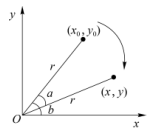
\includegraphics[width=0.32\textheight]{17}
\end{wrapfigure}

设图像上一点$(x_0,y_0)$,$r$为该点到原点的距离,$b$为$r$与$x$轴之间的夹角。$(x_0,y_9)$沿顺时针方向旋转$\alpha$角,变为点$(x,y)$。用矩阵的形式表示为:
$$\begin{pmatrix}x & y & 1\end{pmatrix} = \begin{pmatrix}x_0 & y_0 & 1\end{pmatrix}\begin{pmatrix}cos\alpha & -sin\alpha & 0 \\sin\alpha & cos\alpha & 0 \\0 & 0 & 1 \end{pmatrix}$$

图像的旋转需注意:图像旋转之后,会出现很多的空白点,对这些空白点必须进行填充处理,称这种操作为插值处理。最简单的方法是行插值或列插值:空白点的像素值等于前一点的像素值。

\subsection{图像的形状变换}
图像的形状变换是指用数学模型的方法对图像形状发生的变化进行描述。最基本的形状变换主要包括图像的缩小,放大以及错切等变换。
\subsubsection{图像比例缩小变换}
图像的比例缩小是通过减少像素个数来实现的。需要根据所期望的缩小尺寸,从原图像中选择合适的像素点,使图像缩小之后能够尽量保持原有图像的概貌特征。

基于等间隔采样的图像缩小方法的设计思想是,通过对画面像素的均匀采样来保证所选择到的像素仍可以保持像素的概貌特征。

该方法的具体实现步骤为:设原图像为$F(i,j)$,大小为$M\times N$,其中$i = 1,2,...,M,j=1,2,...,N$。缩小后的图像为$G(i,j)$,大小为$k_1M\times k_2N$,当$k_1=k_2$时为按比例缩小,当$k_1\neq k_2$时为不按比例缩小,且$k_1<1,k_2<1,i=1,2,...,k_1M,j=1,2,...,k_2N$。则有
$$\Delta i=1/k_1, \Delta j=1/k_2$$
$$g(i,j)=f(\Delta i\cdot i,\Delta j\cdot j)$$ 

图像的比例缩小可分为按比例缩小或不按比例缩小。
\begin{figure}[H]
	\centering
	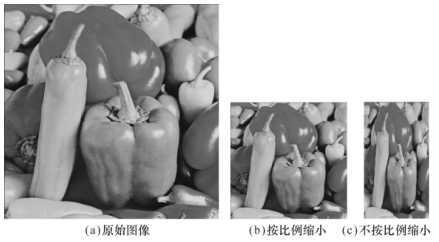
\includegraphics[scale=0.5]{18}
\end{figure}
\subsubsection{图像比例放大变换}
图像的放大是信息的估计问题,需要对尺度放大后多出来的像素位置处填入适当的像素值,比图像的缩小要难。由于图像相邻像素之间的相关性很强,可以利用相关性来实现图像的放大。按比例放大不会引起图像的畸变,而不按比例放大则会产生图像的畸变。

(1)最近领域法

按比例将图像放大k倍,需要将一个像素值添加在新图像的$k\times k$的子块中。假设原图像大小为$3\times 3$,即将一个像素值都赋值给一个像素块。采用最近领域法时,如果放大倍数太大,则会出现马赛克现象。

(2)线性插值法

当求出的分数地址与像素点不一致时,求出周围四个像素点的距离比,根据该比率,由4个领域的像素灰度值进行线性插值。
\begin{figure}[H]
	\centering
	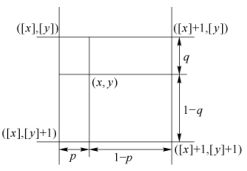
\includegraphics[scale=0.5]{19}
\end{figure}
灰度值的计算公式:$$g(x,y) = (1-q)\{(1-p)\times g([x],[y]) + p\times g([x]+1,[y])\} + q\{(1-p)\times g([x],[y]+1)+p\times g([x]+1,[y]+1)\}$$
\subsubsection{图像错切变换}
图像的错切变换实际上是平面景物在投影平面上的非垂直投影。

(1)水平方向错切

在水平方向上的错切是指图形在水平方向上发生了扭变。图形发生水平方向的错切之后,矩形的水平边扭变成斜边,垂直边不变。

\begin{figure}[H]
	\centering
	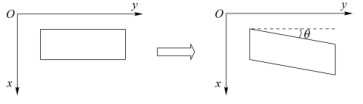
\includegraphics[scale=0.5]{20}
\end{figure}
图像在水平方向上错切的表达式为:
$$\left\{\begin{matrix}
	x'=x + y\tan\theta\\ 
	y'=y
\end{matrix}\right.$$
式中(x,y)为原图像的坐标,(x',y')为错切后的图像坐标。错切后的图形的列坐标不变,行坐标随原坐标(x,y)和系数$\tan\theta$,大于0时,图像沿x轴正方向做错切;小于0时,图像沿x轴负方向做错切。

(2)垂直方向错切

在垂直方向上的错切是指图像在垂直方向上发生扭变。图形发生垂直方向的错切之后,矩形的垂直边扭变为斜边,水平边不变。

\begin{figure}[H]
	\centering
	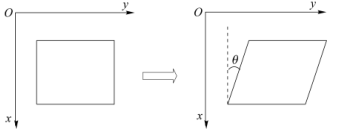
\includegraphics[scale=0.5]{21}
\end{figure}

图像在垂直方向上错切的表达式为:
$$\left\{\begin{matrix}
	x'=x\\ 
	y'=y + x\tan\theta
\end{matrix}\right.$$
式中(x,y)为原图像的坐标,(x',y')为错切后的图像坐标。错切后的图形的列坐标不变,行坐标随原坐标(x,y)和系数$\tan\theta$,大于0时,图像沿y轴正方向做错切;小于0时,图像沿y轴负方向做错切。
\subsubsection{图像的复合变换}
图像的复合变换是指对给定的图像连续实施若干次平移,镜像,旋转,比例缩放等基本变换后完成的变换,又称级联变换。

假设对图像依次进行了基本变换$F_1,F_2,...,F_N$对应的变换矩阵为$T_1,T_2,...,T_N$则图像复合变换的矩阵T表示为
$$T = T_1\cdots T_2\cdots ... \cdots T_N$$

可以做的复合变化如:复合平移,复合旋转,复合缩放。



\subsection{图像的基本统计分析量}
设$f(i,j)$表示大小为$M\times N$的数字图像。
\subsubsection{图像的熵}
一幅图像如果共有k个灰度值,并且各灰度值出现的概率分别为$p_1,p_2,...,p_k$,根据香农定理,图像的平均信息量可计算为:
$$H = -\sum_{i=1}^{k}p_ilog_2p_i$$
H称为熵,当图像中各灰度值出现的概率彼此相等时,则图像的熵最大。
\subsubsection{图像灰度平均值}
灰度平均值是指一幅图像中所有像素灰度值的算术平均值:
$$\bar{f} = \frac{\sum_{i=0}^{M-1}\sum_{j=0}^{N-1}f(i,j)}{MN}$$
图像灰度平均值反映了图像中物体不同部分的平均反射强度。
\subsubsection{图像灰度众数}
图像灰度众数是指图像中出现次数最大的灰度值,其物理意义是指一幅图像中面积占优的物体的灰度值信息。
\subsubsection{图像灰度中值}
图像中值是指数字图像全部灰度级中处于中间的值,当灰度级数为偶数时,则取中间的两个灰度值的平均值。
\subsubsection{图像灰度方差}
灰度方差反映了各像素灰度值与图像平均灰度值的离散程度。
$$S = \frac{\sum_{i=0}^{M-1}\sum_{j=0}^{N-1}[f(i,j)-\bar{f}]^2}{MN}$$
于熵类似,图像灰度方差同样是衡量图像信息量大小的主要度量指标,是图像统计特性中最重要的统计量之一,方差越大,图像的信息量越大。
\subsubsection{图像灰度值域}
图像的灰度值域是指图像最大灰度值$f_{max}(i,j)$和最小灰度值$f_{min}(i,j)$之差。
$$f_{range}(i,j) = f_{max}(i,j) - f_{min}(i,j)$$

\subsection{离散傅里叶变换}
离散傅里叶DFT(Discrete Fourier Transform)变换建立了离散时域(或空域)与离散频域之间的联系。由信号的卷积定理可知,图像信号在时域或空域上处理,计算量会随着离散采样点数的增加而急剧增加。

我们可以将输入的数字信号首先进行DFT,把时域(或空域)中的卷积或相关运算简化为在频域上的相乘操作,然后进行DFT反变换,恢复为时域(或空域)信号。

计算量可大大减少,提高处理速度,另具有快速傅里叶变换(FFT, Fast Fourier Transformer),使计算量减少到直接进行DFT计算的一小部分。


\section{空间域图像增强}
图像的成像,传输或变换过程中,多种因素的影响总会造成图像质量的下降。图像处理的基本目的之一是改善图像质量,而改善图像质量最常用的技术是图像增强。

图像增强是一类基本的图像处理技术,它是指对图像的某些特征如边缘,轮廓,对比度等进行强调,以便于显示,观察或进一步分析与处理。其目的主要有:1.改善图像的视觉效果,提高图像的清晰度。2.将图像转换成一种更适合于人类或机器进行分析处理的形式,以便从图像中获取更有用的信息。

空间域增强法是指直接在图像所在像素空间对像素灰度值进行运算处理。

\subsection{灰度变换}
灰度变换的实质就是按一定的规则修改图像每一个像素的灰度值,从而改变图像灰度的动态范围,属于点运算范畴。

空间域处理基于表达式:
$$g(x,y) = T[f(x,y)]$$
式中,$r$和$s$分别为输入,输出像素的灰度级,T为灰度变换函数的映射关系。灰度变换按映射函数可分为线性变换和非线性变换两种形式。

最小邻域的大小为$1\times 1$。此时, $g$只依赖于点$(x,y)$处的$f$值,而$T$则称为灰度(也称灰度级或映射)变换函数:
$$s = T(r)$$
用$s$和$r$分别表示$g$和$f$在任意点$(x,y)$处的灰度。
\begin{wrapfigure}{r}{4.9cm}
	\centering
	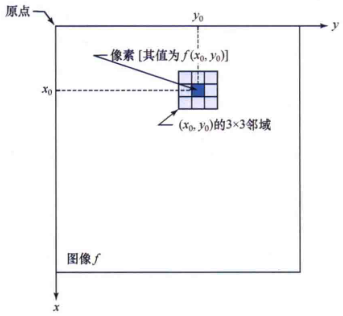
\includegraphics[width=0.23\textheight]{58}
\end{wrapfigure}
将邻域的中心从一个像素移到另一个像素,并将算子$T$应用到邻域中的像素,以便在该位置产生一个输出值。因此,对于任何指定的位置$(x_0,y_0)$,输出图像$g$在这些坐标处的值等于将$T$应用到$f$中原点为$(x_0,y_0)$的邻域的结果。
\begin{figure}[H]
	\centering
	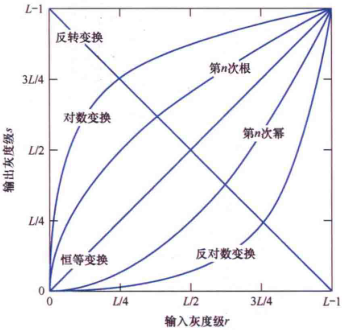
\includegraphics[scale=0.6]{59}
\end{figure}
\subsubsection{灰度线性变换(单像素运算)}
\textbf{图像反转}

将原始图像的灰度值进行反转,使输出图像的灰度随输入图像的灰度增加而减少。
\begin{figure}[H]
	\centering
	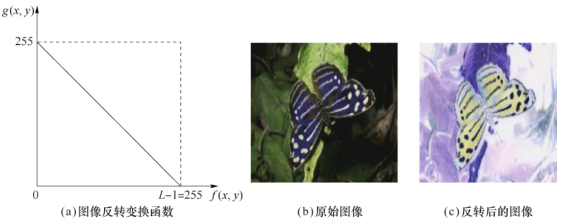
\includegraphics[scale=0.5]{22}
\end{figure}

\textbf{线性变换}

线性变换是对每个线性段逐个像素进行处理,可将原图像灰度值动态范围按线性关系式变换到指定范围。

\begin{figure}[H]
	\centering
	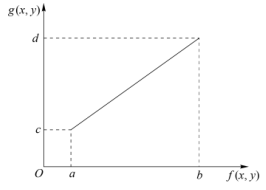
\includegraphics[scale=0.7]{23}
\end{figure}
在曝光不足的情况下,图像灰度可能局限在一个很小的范围内,显示器将显示一个模糊不清,没有灰度层次的图像。采用线性变换对图像的每一个像素灰度做线性拉伸,将有效地改善图像的视觉效果。

\textbf{分段线性变换}

为了突出图像中感兴趣的目标或灰度区间,将图像灰度区间分成两段乃至多段分别作线性变换,称为分段线性变换。

\begin{figure}[H]
	\centering
	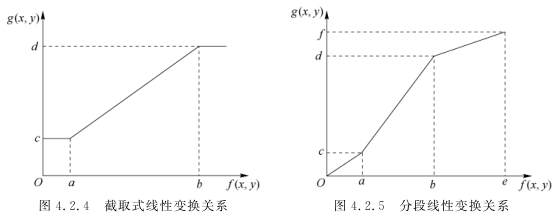
\includegraphics[scale=0.5]{24}
\end{figure}
分段线性变换的优点是可以根据用户的需要,拉伸特征物体的灰度细节,相对抑制不感兴趣的灰度级。

\subsubsection{灰度非线性变换(单像素运算)}
\textbf{对数变换}

对数变换常用来增加低灰度值的像素,扩展低灰度区,压缩高值灰度。当希望对图像的低灰度区进行较大的拉伸而对高灰度区压缩时,可采用这种变换,使图像灰度分布与人的视觉特性相匹配。

对数变换的表达式为$g(x,y) = C * lg[1+|f(x,y)|]$,式中,C为尺度比例常数;$1+|f(x,y)|$是为了避免对零求对数。

\textbf{指数变换}

常用于压缩低灰度值的像素,扩展高灰度区,压缩低值灰度。但由于增强的效果要考虑人的主观感觉,因此不常采用。
\subsubsection{邻域运算}
令$S_{xy}$代表图像$f$中以任意一点$(x,y)$为中心的一个邻域的坐标集。邻域处理在输出图像$g$中的相同坐标处生成一个对应的像素,这个像素的值由输入图像中邻域像素的规定运算和集合$S_{xy}$中的坐标确定。

\subsubsection{图像反转}
得到的灰度级在区间[0,L-1]内的反转图像的形式:
$$s = L - 1 - r$$
采用这种方式反转图像的灰度级,会得到类似照片底片的结果。这种类型的处理可用于增强图像暗色区域中的白色或灰色细节,暗色区域的尺寸很大时这种增强效果更好。
\begin{figure}[H]
	\centering
	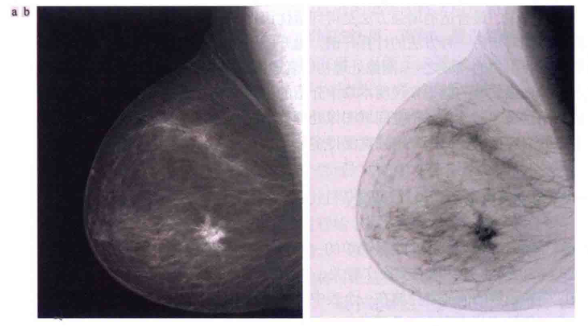
\includegraphics[scale=0.6]{60}
\end{figure}
\subsubsection{对数变换}
对数变换的通式为
$$s = clog(1+r)$$
式中,$c$是一个常数,并假设$r\neg0$。这个变换将输入中范围较窄的低灰度值映射为输出中范围较宽的灰度级。

相反,反对数变换是输入中的高灰度值则被映射为输出中范围较窄的灰度级。我们使用这类变换来扩展图像中的暗像素值,同时压缩高灰度级值。
\subsubsection{幂律(伽马)变换}
幂律变换的形式为:
$$s=cr^\gamma \text{或} s=c(r+\xi)^\gamma$$
式中,$c$和$\gamma$是正常数。考虑到偏移(即输入为0时的一个可度量输出)。幂律曲线用分数值$\gamma$将较窄范围的暗输入值映射为较宽范围的输出值,将高输入值映射为较窄范围的输出值。

用于获取,打印和显示图像的许多设备的响应遵守幂律。用于校正这些幂律响应现象的处理称为伽马校正或伽马编码。

观察发现,当伽马值从0.6降至0.4时,会出现更多的细节。将伽马值进一步减少到0.3,会增强背景中的更多细节,但与开始具有轻微“苍白”外观,对比度开始下降。$\xi = 0.4$时,对比度和可分辨细节的增强效果最好。$\xi =0.3$是一个近似的极限值,低于这个值时,这幅图像的对比度会降低到不可接受的水平。
\subsubsection{分段线性变换函数}
1.对比度拉伸

光照不足,成像传感器的动态范围偏小,图像获取过程中镜头孔径的设置错误等,都可能产生低对比度图像。对应度拉伸可以扩展图像中灰度级范围,使其覆盖记录介质或显示设备的整个理想灰度范围。
\begin{figure}[H]
	\centering
	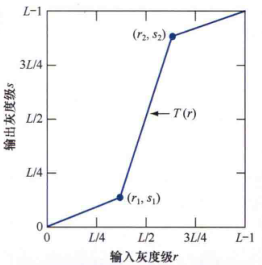
\includegraphics[scale=0.6]{61}
\end{figure}
2.灰度级分层

目的是突出图像中的特定灰度区间。灰度级分层的方法:1.将感兴趣范围内的所有灰度值显示为一个值(如白色),而将所有其他灰度值显示为另一个值(如黑色)。2.使期望的灰度范围变亮(或变暗),但保持图像中的其他灰度级不变。
\begin{figure}[H]
	\centering
	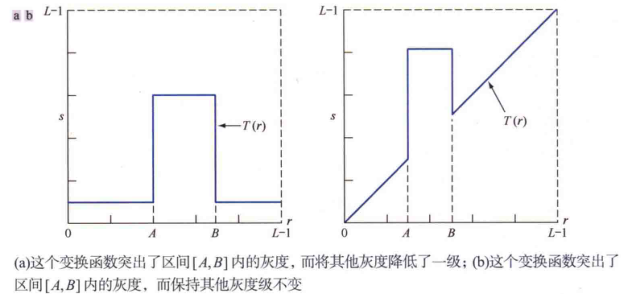
\includegraphics[scale=0.6]{62}
\end{figure}

3.比特平面分层

像素值是由比特组成的整数。例如,在一副256级灰度图像中,图像值是由8比特(1字节)组成。与突出灰度级范围不同的是,我们可以突出特定比特对整个图像外观的贡献。

\begin{figure}[H]
	\centering
	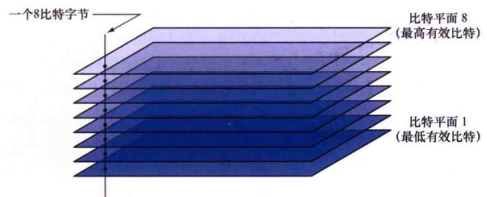
\includegraphics[scale=0.6]{63}
\end{figure}
8比特图像可视为由8个1比特平面组成,其中平面1包含图像中所有像素的最低有效比特,而平面8包含所有像素的最高有效比特。8比特平面中存储4个最高有效比特平面,就能以可接受的细节和色调重建原图像。存储这4个平面而非原图像只需$50\%$的存储容量。

将图像分解成各个比特平面对我们分析图像中每个比特的相对重要性是有用的,这个过程有助于确定量化图像所用比特数的充分性。
\subsection{直方图处理}
图像的直方图是反映一幅图像中的灰度级与出现这种灰度级概率之间关系的图形。
\subsubsection{灰度直方图}
图像的灰度直方图是表示一幅图像灰度分布情况的统计图表,是灰度级的函数,它表示图像中具有每种灰度级的像素的个数。图像直方图的横坐标是灰度级r,纵坐标表示图像中该灰度级的像素的个数$P(r)$。
\begin{figure}[H]
	\centering
	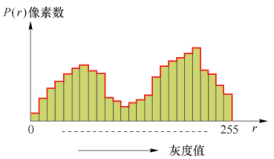
\includegraphics[scale=0.7]{25}
\end{figure}

按照直方图的定义,可表示为:
$$P(r_k) = \frac{n_k}{N} (k=0,1,2...L-1)$$N为一幅图像的总像素数;$n_k$为第k级灰度的像素数;L为灰度级数;$r_k$为第k个灰度级;$P(r_k)$为该灰度级出现的相对频数。

在图像直方图中,r代表图像中像素灰度级,若将其作归一化处理,$0\leq r\leq 1$在灰度级中,$r=0$代表黑,$r=1$代表白。

直方图形状与图像的外观有关。暗图像:大多数直方图容器集中在灰度级的低端。亮图像:大多数直方图容器集中在灰度级的高端。低对比度图像:直方图容器基本位于灰度级的中间。高对比度图像:直方图容器覆盖较宽范围的灰度级,并且像素的分布基本上是均匀的。
\subsubsection{直方图的性质}
1.直方图是图像的一维信息描述。直方图不表示图像的空间信息,只能反映图像的灰度范围,灰度级的分布,整幅图像的平均亮度等信息,而不能反映图像某一灰度值像素所在的位置,因而失去了图像的二维空间信息。

2.任意一幅图像都可以唯一地确定出与其对应的直方图,但不同的图像可能有相同的直方图。

\subsection{空间滤波}
空间滤波是在图像空间中借助模板进行邻域操作完成的(即通过把每个像素的值替换为改像素及其邻域的函数值来修改图像),是图像处理邻域应用广泛的主要工具之一。空间滤波按线性和非线性的特点有:基于傅里叶变换分析的线性滤波器和直接对邻域进行操作的非线性空间滤波器。

空间滤波根据功能主要分为平滑滤波和锐化滤波两种。平滑滤波的目的是消除噪声。去除太小的细节或将目标内的小间断连接起来实现模糊。锐化滤波的目的是为了增强被模糊的细节。

\subsubsection{空域的邻域操作}
空间滤波的原理是利用模板进行卷积运算,即将图像模板下的像素与模板系数的乘积求和操作。主要步骤:

\noindent 1.在待处理的图像中逐点移动模板,使模板在图中遍历漫游全部像素(除达到的边界之外),并将模板中心与图像中某个像素位置重合;

\noindent 2.将模板上系数与模板下对应像素相乘;

\noindent 3.将所有乘积相加;

\noindent 4.将模板的输出响应乘积

\subsubsection{空域中利用模板求卷积运算}
卷积操作实际上就是利用模板对图像进行领域操作。输出图像中每一个像素的取值都是通过模板对输入像素相应邻域内的像素灰度值进行加权和的操作。具体的权值可以通过卷积核(也称滤波器)进行定义。

\subsection{空间平滑滤波}
图像平滑的主要目的是减少图像噪声。实际应用中获得的图像都因受到干扰而含有噪声,噪声产生的原因决定了噪声分布的特性及其图像信号的关系。图像平滑总是以一定的细节模糊为代价。

一般图像处理技术常见的噪声有:

(1)加性噪声:如图像传输过程中引进的“信道噪声”

(2)乘性噪声:与图像信号相关,信号和噪声成正比

(3)量化噪声:数字图像的主要噪声源,其大小显示出数字图像和原始图像的差异。减少这种噪声的最好方法就是采用按灰度级概率密度函数选择量化级的最优量化措施。

(4)椒盐噪声:如图像切割引起的黑图像上的白点噪声,白图像上的黑点噪声,以及在变换域引入的噪声,使图像逆变换噪声等

将空间域模板用于图像处理,通常称为空间滤波,空间域模板称为空间滤波器。空域平滑滤波包括邻域平均法(线性)和中值滤波法(非线性)

\subsubsection{邻域平均法(均值滤波法)}
在图像空间,假定有一幅$N\times N$个像素的原始图像$f(x,y)$,用领域内几个像素的平均灰度值去代替图像中的每一个像素点值的操作,经过平滑处理后得到一幅图像。

选取算子的原则是必须保证全部权系数之和为单位值,即无论如何构成模板,整个模板的平均数为1,且模板系数都为正数。不同的算子,其中心或邻域的重要程度不同。

\begin{figure}[H]
	\centering
	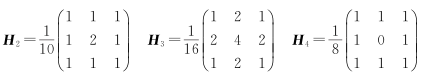
\includegraphics[scale=0.7]{26}
\end{figure}

\subsubsection{中值平均法}
领域平均法在消除噪声的同时会使图像中的一些细节模糊,故可使用中值滤波法。中值滤波器的输出像素是由邻域像素的中间值而不是平均值决定的。中值滤波器模数较少,更适合于消除图像的孤立噪声点。

通常窗口内像素为奇数,以便于有中间像素。若窗口内像素为偶数时,则中值取中间两像素灰度值的平均值。

中值滤波法的主要步骤:1.将模板在图中漫游,并将模板中心与图中的某个像素位置重合;2.读取模板下各对应像素的灰度值;3.将模板对应的像素灰度值进行从小到大排序;4.选取灰度序列里排在中间的1个像素的灰度值;5.将这个中间值赋值给对应模板中心位置的像素作为像素的灰度值。

\begin{figure}[H]
	\centering
	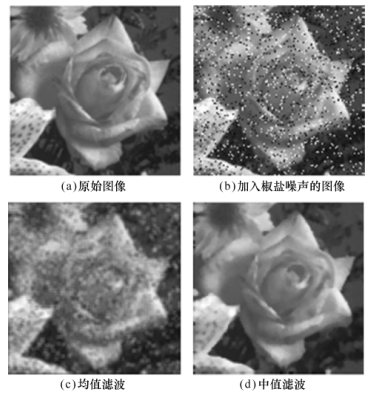
\includegraphics[scale=0.5]{3}
\end{figure}

\subsection{空间锐化滤波}
图像锐化的目的是为了突出图像的边缘信息和线条,加强图像的轮廓特征,使图像的边缘,细节,轮廓变清晰,以便于人眼的观察和机器的识别。图像的边缘和轮廓一般位于图像灰度突变的地方,因此可以用差分提取边缘和轮廓并进行增强。

\begin{figure}[H]
	\centering
	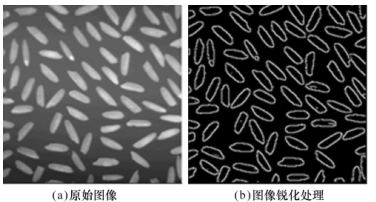
\includegraphics[scale=0.5]{27}
\end{figure}

\subsubsection{梯度运算}
水平垂直差分法:对一幅图像施加梯度模算子,可以增加灰度变化的幅度,而且该算子具有各向同性和位置不变性的特点。为了降低运算量并且保持灰度的相对变化,在实际计算中常用绝对值代替平方和平均根运算来近似计算梯度的幅值。

罗伯茨交叉差分算法:所有梯度值都和相邻像素之间的灰度值成比例。因此在灰度变化比较大的边缘轮廓点处有较大的梯度值,而在灰度变化比较平缓的区域,相应的梯度值也较小。

\begin{figure}[H]
	\centering
	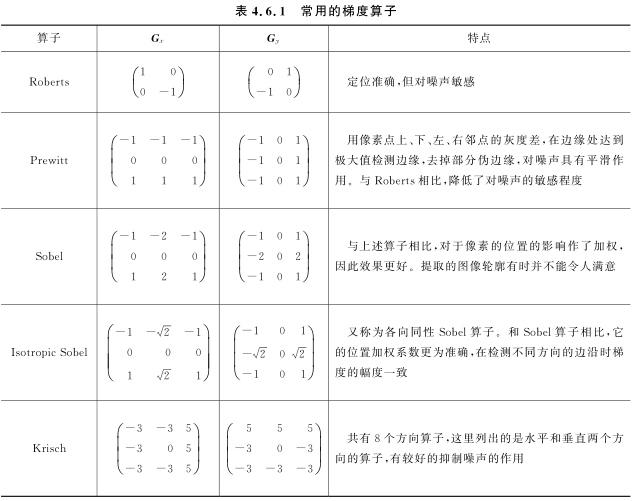
\includegraphics[scale=0.5]{28}
\end{figure}

\subsubsection{拉普拉斯运算}
拉普拉斯算子是具有各向同性的二阶微分算子,一个连续的二元函数$f(x,y)$,它在位置$(x,y)$处的拉普拉斯运算定义为:
$$\bigtriangledown^2f(x,y) = \frac{\partial^2f}{\partial x^2}+\frac{\partial^2f}{\partial y^2}$$

\subsection{空域伪彩色增强}
伪彩色增强是指把灰度图像或者多波段图像变换成彩色图像的技术过程,主要是对原来灰度图像中不同灰度值的区域赋予不同的颜色以便更明显地区分它们。分层越多,彩色越多。

\subsubsection{灰度分层法}
灰度分层法又称为灰度分割法或密度分层法,是伪彩色图像增强技术中最基础,最简单的方法。

设一幅灰度图像$f(x,y)$,在,某一灰度级如$f(x,y)+l_1$上设置一个平行于$xy$平面的切面。这幅灰度图像被分成只有两个灰度级,对于切面以下的,即灰度级小于$l_1$的像素分配一种颜色;相应地,对于切面以上地,即灰度级大于$l_1$地像素分配另一种颜色。

若将以上图像地灰度级用$M$个切割平面去分层,就会得到$M$个不同灰度级地区域$S_1,S_2,...,S_M$。d对这M个区域中地像素人为地分配M个不同地颜色,就可以得到具有M种颜色的伪彩色图像。灰度层次技术的效果与分割层数成正比,层次越多,细节越丰富,彩色越柔和,但分割的层数受显示系统的硬件性能约束。

\subsubsection{灰度变换法}
其方法是先将灰度图像$f(x,y)$送入具有不同变换特征的红,绿,蓝3个变换器,然后再将3个变换器的不同输出$I_R(x,y),I_G(x,y),I_B(x,y)$分别送到彩色显像管的红,绿,蓝电子枪。这里受调制的是像素的灰度值而不是像素的位置。对于同一个灰度级而言,由于3个变换器对其实施不同的变换,因而3个变换器的输出不同,从而再彩色显像管里合成某一种彩色。不同大小灰度级可以合成不同彩色。

\begin{figure}[H]
	\centering
	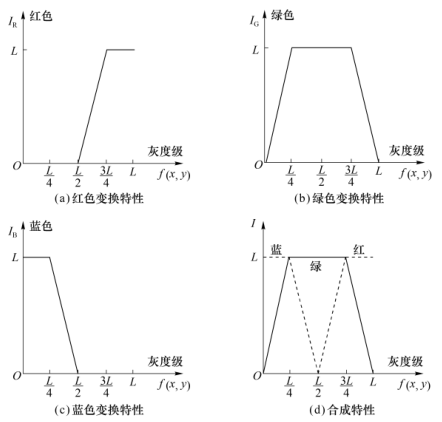
\includegraphics[scale=0.5]{29}
\end{figure}

\section{频率域图像增强}
将图像的特征在变换域种表现出来,特别是那些空间法无法完成的一些特殊处理,将空间域的处理转换为变换域的处理,不仅可以减少计算量,而且还可以获得更有效的处理,最后再变换回到空间域以得到所需的效果。

由于一般图像信号是二维信号,因此处理图像信号的系统也常常是二维的系统。在各种不同的二维图像处理系统模型中,线性移位不变系统模型最为简单,但基本能够反映该系统的主要性能,应用最为广泛。

\subsection{二维线性不变系统}
二维线性系统:设$L[\cdot]$为二维系统对输入信号$\cdot$的响应。满足以下线性运算关系:
$$
\begin{cases}
	& L[f_1(x,y)+f_2(x,y)] = L[f_1(x,y)]+L[f_2(x,y)] \\ 
	& L[af(x,y)] = aL[f(x,y)]
\end{cases}
$$
式中,a为任意常数。

二维线性移位不变系统(Shift Invariant System):系统对输入信号f(x,y)的响应为$L[f(x,y)]=g(x,y)$,当输入信号$f(x,y)$位移$\alpha,\beta$单位后,若系统的响应同样也位移$\alpha,\beta$单位,为$L[f(x-\alpha,y-\beta)] = g(x-\alpha,y-\beta)$

当二维线性系统的输入为单位冲击函数$\delta(x,y)$时,系统封的输出称为冲激响应,用h(x,y)表示,由于h(x,y)是当系统的输入为$\delta$函数或理想点光源时的系统输出,是对点光源的响应,因此也称之为点扩展函数(PSF, Point Spread Function)。

$\delta$函数经过理想的图像系统后的点扩展函数h(x,y),仍然能保持它的单位冲激特性。而质量差的图像系统h(x,y)会把图像中的$\delta$函数在其中心点处弥散开来。
\subsection{二维离散傅里叶变换}
对一个连续函数$f(x,y)$等间隔采样可得到1个离散矩阵序列,设以$M\times N$长方形网格采样,共采用了$M\times N$个样本。

其二维离散傅里叶变换定义为:
$$F(u,v) = \sum_{x=0}^{M-1}\sum_{y=0}^{N-1}f(x,y)e^{-j2\pi(\frac{ux}{M}+\frac{vy}{N})},\quad u=0,1,...,M-1; v= 0,1,...,N-1$$
其逆变换定义为:
$$f(x,y) =\frac{1}{MN} \sum_{x=0}^{M-1}\sum_{y=0}^{N-1}F(u,v)e^{j2\pi(\frac{ux}{M}+\frac{vy}{N})},\quad u=0,1,...,M-1; v= 0,1,...,N-1$$

通常在图像处理种,一般总是选择方阵列,即$M=N$

对大多数无明显颗粒噪声的图像来说,低频区域集中了$85\%$的能量。如果变换后仅传递低频分量的幅值,对高频分量不传送,逆变换前将它们恢复为零值,就可以达到压缩的目的。

图像灰度变化缓慢的区域,对应它变换后的低频分量部分;图像灰度呈现阶跃变化的区域,对应变换后的高频分量部分。
\subsection{离散余弦变换}
如果函数$f(x)$为一个连续的实偶函数。则此函数的傅里叶变换如下:
$$F(u) = \int_{-\infty}^{\infty}f(x)e^{-j2\pi ux}dx = \int_{-\infty}^{\infty}f(x)cos(2\pi ux)dx - j\int_{-\infty}^{\infty}f(x)sin(2\pi ux)dx = \int_{-\infty}^{\infty}f(x)cos(2\pi ux)dx$$

因为虚部的被积项为奇函数,故傅里叶变换的虚数项为零,由于变换后的结果仅含有余弦项,故称为余弦变换。

\subsubsection{一维离散余弦变换}
离散余弦变换也是一种可分离的变换,设${f(x)|x=0,1,2,...,N-1}$为离散的信号序列,一维DCT变换对定义如下:
$$C(u) = a(u)\sum_{x=0}^{N-1}f(x)cos\frac{(2x+1)u\pi}{2N}\qquad (u=0,1,2,...,N-1)$$
$$f(x) = \sum_{u=0}^{N-1}a(u)C(u)cos\frac{(2x+1)u\pi}{2N}\qquad (x=0,1,2,...,N-1)$$
式中
$$a(u) = \left\{\begin{matrix}
	\sqrt{1/N} u=0\\ 
	\sqrt{2/N} \text{其他}
\end{matrix}\right.$$
\subsubsection{二维离散余弦变换}
设$f(x,y)$为$N\times N$的数字图像矩阵,则二维DCT变换对定义如下:
$$C(u,v) = a(u)a(v)\sum_{x=0}^{N-1}\sum_{y=0}^{N-1}f(x,y)cos\frac{(2x+1)u\pi}{2N}cos\frac{(2y+1)v\pi}{2N}$$
式中,$u,v=0,1,2,...,N-1$
$$f(x,y) = \sum_{x=0}^{N-1}\sum_{y=0}^{N-1}a(u)a(v)C(u,v)cos\frac{(2x+1)u\pi}{2N}cos\frac{(2y+1)v\pi}{2N}$$
式中,$u,v=0,1,2,...,N-1$

DCT的计算速度快,已广泛应用于数字信号处理中,例如图像压缩编码,语言信号处理。
\subsubsection{离散余弦变换的应用}
图像压缩:目前的国际压缩标准JPEG格式种就用到了DCT变换。具体做法:给高频系数部分大间隔量化,低频系数部分小间隔量化。它比傅里叶变化有更强的信息集中能力,可以提高编码效率。

具体在JPEG图像压缩算法中,首先将输入图像划分为$8\times8$的方块,然后对每个方块执行二维离散余弦变换,最后将变换得到量化的DCT系数进行编码和传送,形成压缩后的图像格式。在接收端,将量化的DCT系数进行解码,并对每个$8\times 8$方块进行二维IDCT,最后将操作完成后的块组合成一幅完整的图像。
\subsection{二维离散卷积}
1.一维离散卷积

输入信号f(x)通过一维线性时不变系统后,输出g(x)为输入信号f(x)和系统冲激响应h(x)的离散卷积,定义为:
$$g(x)=f(x)*h(x)=\sum_{i=0}^{M-1}f(i)h(x-i)$$

离散卷积和连续卷积之间的误差仍然主要取决于时域和频域的取样间隔,只有取样间隔充分小,离散卷积完全有可能充分逼近相应的连续卷积,离散卷积带来的误差就可以忽略。

2.一维卷积的矩阵表示

将输入,输出信号分别表示成M维列向量,$f=[f(0) f(1) ... f(M-1)]^T, g=[g(0) g(1) ... g(M-1)]^T$。用系统响应h(x)函数构造出矩阵H(系统矩阵),是卷积运算能用矩阵方式表示。系统响应的矩阵表达式为$g=H\bullet f$。

由于$h(x)$为周期函数,$h(M+x)=h(x)$,M是其周期。

$$\begin{aligned}
	\begin{bmatrix} 
		g(0)\\g(1)\\\vdots\\g(M-1) \end{bmatrix}&= \begin{bmatrix}
		h(0) & h(-1) & h(-2) & \cdots & h(-M+1) \\
		h(1) & h(0) & h(-1) & \cdots & h(-M+2) \\
		\vdots & \vdots & \vdots & \ddots & \vdots \\
		h(M-1) & h(M-2) & h(M-3) & \cdots & h(0)
	\end{bmatrix}\cdot \begin{bmatrix} 
		f(0)\\f(1)\\\vdots\\f(M-1) \end{bmatrix} \\ &=\begin{bmatrix}
		h(0) & h(M-1) & h(M-2) & \cdots & h(1) \\
		h(1) & h(0) & h(M-1) & \cdots & h(2) \\
		\vdots & \vdots & \vdots & \ddots & \vdots \\
		h(M-1) & h(M-2) & h(M-3) & \cdots & h(0)
	\end{bmatrix}\cdot \begin{bmatrix} 
		f(0)\\f(1)\\\vdots\\f(M-1) \end{bmatrix}
\end{aligned}$$

3.二维离散卷积

f(x,y)为$m\times n$点,补零后成为
$$f_e(x,y)=\left\{\begin{matrix}
	f(x,y), 0\leq x\leq m-1 \text{且} 0\leq y\leq n-1\\ 
	0, m\leq x\leq M-1\text{或}n\leq y\leq N-1
\end{matrix}\right.$$

h(x,y)为$m\times n$点,补零后成为
$$h_e(x,y)=\left\{\begin{matrix}
	h(x,y), 0\leq x\leq p-1 \text{且} 0\leq y\leq q-1\\ 
	0, p\leq x\leq M-1\text{或}q\leq y\leq N-1
\end{matrix}\right.$$

将其补零之后的二维卷积运算如下:
$$g_e(x,y)=f_e(x,y)*h_e(x,y)=\sum_{i=0}^{M-1}\sum_{j=0}^{N-1}f_e(i,j)\cdot h_e(x-i,y-j)$$

4.二维卷积的矩阵表示

在二维情况下只讨论方阵,M=N,二维卷积的矩阵表示和一维时一样。
$$g = H\cdot f$$
$g$表示输出矩阵堆叠成的列矢量,$f$为输入矩阵堆叠的列矢量。

将输入矩阵(图像)变为列矢量的具体方法是将$f$矩阵每一行的N个像素拉成一列,共N列,顺序堆叠,形成一个$N^2$维的列向量。 

\subsection{频率滤波}
在具体的图像增强应用中,$f(x,y)$是给定的,主要步骤:1.计算需要增强的图像$f(x,y)$的傅里叶变换$F(u,v)$2.将其与1个传递函数$H(u,v)$相乘3.再将结果进行傅里叶逆变换,就可以得到增强的图像$g(x,y)$

\subsubsection{频率低通平滑滤波}
在分析图像信号的频率特性时,对于一幅图像,直流分量代表了图像的平均灰度,大面积的背景区域和缓慢变化部分则代表图像的低频分量,而它的边缘,细节,跳跃部分以及颗粒噪声都代表图像的高频分量。
\begin{figure}[H]
	\centering
	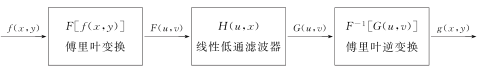
\includegraphics[scale=0.7]{30}
\end{figure}

1.\textbf{理想低通滤波器(ILPF)}

\begin{wrapfigure}{r}{5cm}
	\centering
	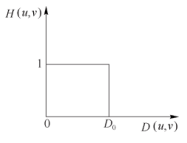
\includegraphics[width=0.23\textheight]{31}
\end{wrapfigure}
二维理想低通滤波器如图,它的传递函数$H(u,v)$为
$$H(u,v) = \left\{\begin{matrix}
	1 \qquad D(u,v)\leq D_0\\ 
	0 \qquad D(u,v)>D_0
\end{matrix}\right.$$
式中,$D_0$为理想低通滤波器的截至频率,是一个规定非负的量。$D_0$也称为截至频率。这种理想低通滤波器尽管在计算机中可以模拟实现,但理想低通滤波器无法用实际的电子器件硬件实现这种从1到0陡峭突变的截至频率。

2.\textbf{巴特沃斯低通滤波器(BLPF)}

\begin{wrapfigure}{r}{5cm}
	\centering
	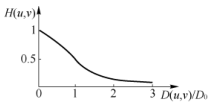
\includegraphics[width=0.23\textheight]{32}
\end{wrapfigure}
n阶巴特沃斯(Butterworth)低通滤波器,传递函数:
$$H(u,v) = \frac{1}{1+[D(u,v)/D_0]^{2n}}$$
当$D(u,v)=D_0, n=1$时,$H(u,v)$在$D_0$处的值降为其最大值的1/2。

另一种巴特沃斯低通滤波器传递函数为:
$$H(u,v) = \frac{1}{1+(\sqrt{2}-1)[D(u,v)/D_0]^{2n}}$$
当$D(u,v)/D_0=1,n=1$时,$H(u,v)$在$D_0$处的值为其最大值的$\frac{1}{\sqrt{2}}$

巴特沃斯低通滤波器传递函数特性为连续性衰减,不像理想低通滤波器时陡峭和明显的不连续性衰减。在它的尾部保留有较多的高频,所以对噪声的平滑效果不如理想低通滤波器。采用该滤波器在抑制噪声的同时,图像边缘的模糊程度大大减少,振铃效应不明显。

3.\textbf{指数低通滤波器(ELPF)}

\begin{wrapfigure}{r}{5.5cm}
	\centering
	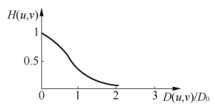
\includegraphics[width=0.23\textheight]{33}
\end{wrapfigure}
传递函数为:
$$H(u,v) = exp\{-[D(u,v)/D_0]^n\}$$
或

$$H(u,v) = exp\{ln(1/\sqrt{2})[D(u,v)/D_0]^n\}$$
式中$D_0$为截止频率,$n$为阶数。上式两式的衰减特性不同。由于ELPF具有比较平滑的过渡带,经此平滑后的图像没有“振铃”现象,而与巴特沃斯滤波相比,它具有更快的衰减特性,处理的图像稍微模糊一些。

4.\textbf{梯形低通滤波器(TLPF)}

\begin{wrapfigure}{r}{5.5cm}
	\centering
	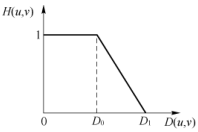
\includegraphics[width=0.23\textheight]{34}
\end{wrapfigure}
传递函数:
$$H(u,v) = \left\{\begin{matrix}
	&1 \qquad D(u,v)< D_0\\ 
	&\frac{D(u,v)-D_1}{D_0-D_1} D_0\leq D(u,v)\leq D_1 \\
	&0 \qquad D(u,v)> D_1
\end{matrix}\right.$$
式中,$D_1$为梯形低通滤波器的截止频率。$D_0$和$D_1$按要求预想指定为$D_0<D_1$,它的性能介于理想低通滤波器与巴特沃斯低通滤波器之间,对图像有一定的模糊和振铃效应。

\subsubsection{频率高通锐化滤波}
由于图像种的边缘,线条等细节部分与图像频率中高频分量相对应,在频率中用高通滤波器处理,能够使图像的边缘或线条变得清晰,图像得到锐化。

在频率中实现高通滤波,其数学表达式为:
$$G(u,v) = F(u,v) \cdot H(u,v)$$
式中,$F(u,v)$为原图像$f(x,y)$的傅里叶频谱;$G(u,v)$为锐化后图像$g(x,y)$的傅里叶频谱;$H(u,v)$为滤波器的转移函数(即频谱响应)。

1.\textbf{理想高通滤波器(IHPF)}
二维理想高通滤波器的传递函数$H(u,v)$定义为:
$$H(u,v) = \left\{\begin{matrix}
	&1 \qquad D(u,v)>D_0\\
	&0 \qquad D(u,v)\leq D_0
\end{matrix}\right.$$
式中,$D_0$为截止频率。$D(u,v)=\sqrt{u^2+v^2}$是频率平面点$(u,v)$到频率平面原点$(0,0)$的距离。

它的形状上和理想低通滤波器的形状刚好相反,但与理想低通滤波器一样,这种理想高通滤波器也无法用实际的电子器件硬件来实现。

2.\textbf{巴特沃斯高通滤波器(BHPF)}
n阶巴特沃斯高通滤波器的传递函数为:
$$H(u,v) = \frac{1}{1+[D_0/D(u,v)]^{2n}}$$
式中,$D_0$为截止频率,$D(u,v)=\sqrt{u^2+v^2}$为点$(u,v)$到频率平面原点的距离。当$D(u,v)=D_0$时,$H(u,v)$下降到最大值的$1/2$

当选择截止频率$D_0$,要求使该点处的$H(u,v)$下降到最大值的$1/\sqrt{2}$为条件时,可用下式实现:
$$H(u,v) = \frac{1}{1+(\sqrt{2}-1)[D_0/D(u,v)]^{2n}}$$

3.\textbf{指数型高通滤波器(EHPF)}
指数型高通滤波器的传递函数为:
$$H(u,v) = e^{-[D_0/D(u,v)]^n}$$
式中,$D_0$为截止频率,变量$n$控制着从原点算起的距离函数$H(u,v)$的增长率。当$D(u,v)=D_0$时,$H(u,v)$下降到最大值的$1/e$

当选择截止频率$D_0$,要求使该点处的$H(u,v)$下降到最大值的$1/\sqrt{2}$为条件时,可用下式实现:
$$H(u,v) = e^{ln(1/\sqrt{2})[D_0/D(u,v)]^n}$$

4.\textbf{梯形高通滤波器(THPF)}
梯形高通滤波器的传递函数:
$$H(u,v) = \left\{\begin{matrix}
	&0 \qquad D(u,v)< D_1\\ 
	&\frac{D(u,v)-D_1}{D_0-D_1} D_1\leq D(u,v)\leq D_0 \\
	&1 \qquad D(u,v)> D_0
\end{matrix}\right.$$
式中,$D_0$为梯形高通滤波器的截止频率。$D_1$为0截止频率,频率低于$D_1$的频率全部衰减。只要满足条件$D_0>D_1$即可。

\subsubsection{频率伪彩色增强}
频率伪彩色处理首先把灰度图像经傅里叶变换到频率域,在频率域内用3个不同传递特性的滤波器将其分离成3个独立分量,从3个不同频率的滤波器输出的信号在经过傅里叶逆变换,可以对这3幅图像再作后期处理,最后把它们作为三基色分量分别加到彩色显示器的红,绿,蓝显示通道,从而实现频率域的伪彩色处理。

\begin{figure}[H]
	\centering
	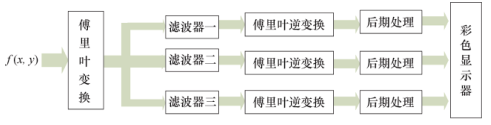
\includegraphics[scale=0.5]{35}
\end{figure}

这种方法的基本思想是根据图像中各区域的不同频率含量给区域赋予不同颜色。为得到不同的频率分量可分别使用低通,带通(或带组)和高通滤波器作为上图的3个滤波器。如果希望图像的边缘(即高频分量)成为红色,则可以将红色通道滤波器设计成高通滤波器。如果希望抑制图像中的某种频率成分,则可以把此频率的滤波器设计成带阻滤波器。

\section{图像压缩编码}
随着信息社会的飞速发展,图像数据的存储和传输技术扮演着越来越重要的角色,特别是网络和通信技术的发展使得图像的存储,处理和传输问题更加突出,数据压缩技术成为数字图像处理中的关键技术。
\subsection{图像压缩编码概述}
图像压缩主要研究图像数据的表示,传输,变换和编码方法,目的是减少存储数据所需的空间和传输数据所用的时间。总体说,就是利用图像数据固有的冗余性和相关性,对图像数据按一定的规则将一个大的数据文件转换成较小同性质文件的变换和组合,从而达到以尽可能少的符号来表示尽可能多的信息的目的。
\subsubsection{数据压缩的基本概念}
\begin{figure}[H]
	\centering
	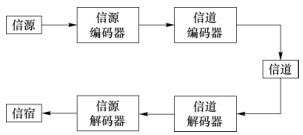
\includegraphics[scale=0.5]{36}
\end{figure}
数据压缩处理是由编码和解码两个过程组成的,包括信源,信源编码器,信道编码器,信道,信道解码器,信源解码器,新宿几个组成部分。编码是对原始的信源数据进行压缩,便于传输或存储;解码是编码的反过程,它将不能被信宿直接使用的数据还原成可用的数据。

信源编码器用于消除或减少输入的冗余信息,主要解决压缩的有效性问题,而信道编码器用于提高传输的抗干扰能力,主要解决编码的可靠性问题。

信息论中,以熵为代表信源所含的平均信息量,若信源编码的熵大于信源的实际熵,则信源中的数据一定存在冗余度。在实际应用场合,压缩过程应尽量保证去除冗余量而不会或较少地减少信息量,即压缩后地数据要能够完全或一定地容差内近似恢复。

\subsubsection{图像压缩编码地必要性}
一幅分辨率为640像素$\times$480像素地彩色图像(24bit/pixel),其数据量约为921.6KB。如果以每秒30帧地速度播放,则每秒地数据量为:$640x480x24x30 bit = 221Mbit$,需要$221Mbit/s$的通信回路;

如果存放在650MB的光盘中,在不考虑音频信号的情况下,每张光盘也只能播放24秒。

从本质上来说,图像压缩编码就是对要处理的图像数据按照一定的规则进行变换和组合,从而达到尽可能少的数据来表示尽可能多的数据信息的目的。

\subsubsection{图像压缩编码的可能性}
图像数据本身固有的冗余性和相关性,使得将一个大的图像数据文件转换成较小的图像数据文件成为可能,图像数据压缩就是要去掉图像信号数据的冗余性。

1.空间冗余(像素间冗余,几何冗余):
在同一幅图像中,规则物体和规则背景的表面物理特性具有相关性,这些相关性的光成像结果在数字化图像中就表现为数据冗余。

2.信息熵冗余(编码冗余):
如果图像中平均每个像素使用的比特数大于该图像的信息熵,则图像中存在的冗余称为信息熵冗余。

3.结构冗余
有些图像存在较强的纹理结构,称为结构冗余。

4.知识冗余
对某些图像的理解与某些知识有相当大的相关性。有些规律性的结构可由先验知识和背景知识得到,称为知识冗余。

5.心理视觉冗余
有些信息在视觉感觉过程中与另外一些信息相比并不那么重要,这些信息可认为是心理视觉冗余的,去除这些信息并不会明显地降低所感受到的图像的质量。心理视觉冗余的存在是与人观察图像的方式有关的,人的观察图像时主要是寻找某些比较明显的目标特征,而不是定量地分析图像中每个像素的亮度。

\subsubsection{图像压缩编码的分类}
(1)根据解压重建后的图像和原始图像之间是否有误差,图像编码压缩分为无损(无失真,无误差,信息保持型)编码和有损(有失真,有误差,信息非保持型)编码两大类。

1.无损编码:这类压缩算法中删除的仅仅是图像数据中冗余的信息,因此在解压缩时能精确地恢复原始图像。无损编码用于要求重建后预想严格地与原始图像保持相同地场合。

2.有损编码:把不相干地信息也删除了,因此在解压缩时只能对原始图像进行近似地重建,而不能精确地复原,有损编码适合大多数用于存储数字化地模拟数据。

(2)根据编码原理,图像压缩编码分为熵编码,预测编码,变换编码和混合编码

1.熵编码:这是纯粹基于信号统计特性地编码技术,是一种无损压缩。熵编码地基本原理是对于出现概率较大地符号赋予一个短码字,而对出现概率较小地符号赋予一个长码字,从而使得最终地平均码字达到最小。常见地熵编码有霍夫曼编码,算术编码和行程编码。

2.预测编码:基于图像数据的空间或时间冗余特性,用相邻的已知像素(或像素块)来预测当前像素(或像素块)的取值,然后再对预测误差进行量化和编码。预测编码可分为帧内预测和帧间预测,常见的预测编码有差分脉冲编码调制(differential Pulse Code Modulation,DPCM)和运动补偿法。

3.变换编码:通常将空间域上的图像经过正交变换映射到另一个变换域上,使变换后的系数之间的相关性降低。图像变换本身并不能压缩数据,但变换后图像的大部分能量只集中到少数几个变换系数熵,再采用适当的量化和熵编码就可以有效地压缩图像。

4.混合编码:综合了熵编码,变换编码或预测编码地编码方法,如JPEG标准和MPEG标准。

\subsubsection{图像压缩编码的技术指标}
图像编码地结果减少了数据量,所以适合存储和传输,但实际应用时需要恢复图像形式才能使用。对于图像编码地质量评价主要体现在基于压缩编码参数地评价和基于保真度准则的评价。

(1).基于压缩编码参数的评价

1.信息量,信息熵,平均码长:

令图像像素灰度级集合为${l_1,l_2,...,l_m}$,其对应的概率分别为$p(l_1),p(l_2),...,p(l_m)$根据香农信息论,定义其信息量为:
$$I(l_i) = -log_2p(l_i) (i=1,2,...,m)$$
如果将图像所有可能灰度级的信息进行平均,就得到信息熵,也就是平均信息量。

信息熵定义为:
$$H = \sum_{i=1}^{m}p(l_i)I(l_i) = -\sum_{i=1}^{m}p(l_i)log_2p(l_i)$$
式中,H的单位是比特/字符。图像的信息熵表示图像灰度级集合的比特数的均值,或者说描述了图像信源的平均信息量。

信息熵是进行无失真编码的理论极限,低于此极限的无失真编码方法是不存在的。当灰度级集合${l_1,l_2,...,l_m}$中$l_i$出现的概率相等,都为$2^{-L}$时,熵H最大,等于L比特;只有当$l_i$出现的概率不相等时,H才会小于L。

平均码长定义为:
$$\bar{L} = \sum_{i=1}^{m}n_ip(l_i)$$
式中,$n_i$为灰度级$l_i$所对应的编码码字长度,平均码长的单位也是比特/字符。

2.编码效率,冗余度

编码效率定义为:
$$ \eta = \frac{H}{\bar{L}}$$
如果$\bar{L}$与$H$相等,编码效果最佳;如果$\bar{L}$与$H$接近,编码效果佳;如果$\bar{L}$远大于$H$,编码效果差;

如果编码效率$\eta \neq 100\%$,就说明还有冗余度。冗余度定义为:
$$r = 1 - \eta$$
r越小,说明可压缩的余地越小。

总之,一个编码系统要研究的问题是设法减少编码平均长度,使得编码效率尽量趋于$100\%$,而冗余度尽量趋于0。

3.压缩比

压缩比$C_r$是衡量数据压缩方法的压缩程度的一个指标,反映压缩效率。$C_r$定义为压缩前图像每像素码长的平均码长与压缩后每像素码长的平均码长之比,即
$$c_r = \frac{\sum_{i=1}^{M}\sum_{j=1}^{N}r_b(i,j)}{\sum_{i=1}^{M}\sum_{j=1}^{N}r_c(i,j)} = \frac{\bar{r_b}}{\bar{r_c}}$$
式中,图像的尺寸为$M\times N$,$r_b$为原图像像素使用的码长,$r_c$为压缩后的图像像素使用的码长,$\bar{r_b}$为原图像像素使用的平均码长,$\bar{r_c}$为压缩后每像素使用的平均码长。 

(2).基于保真度准则的评价
描述解码图像相对于原始图像偏离程度的测度一般称为保真度准则。常用的准则分为客观保真度准则(均方根误差,均方根信噪比,峰值信噪比)和主观保真度

1.均方根误差$e_{rms}$
假设$f(x,y)$代表输入图像,$\hat{f}(x,y)$代表对$f(x,y)$先压缩又解压缩后得到的$f(x,y)$的近似,对任意的给定点$(x,y)$,$f(x,y)$和$\hat{f}(x,y)$之间的误差定义为:
$$e(x,y) = \hat{f}(x,y) - f(x,y)$$
如果两幅图片的尺寸均为$M\times N$总误差为
$$\sum_{x=0}^{M-1}\sum_{y=0}^{N-1}[\hat{f}(x,y) - f(x,y)]$$
$f(x,y)$和$\hat{f}(x,y)$之间的均方根误差$e_{rms}$为:
$$e_{rms} = {\frac{1}{MN}\sum_{x=0}^{M-1}\sum_{y=0}^{N-1}[\hat{f}(x,y) - f(x,y)]^2}^{1/2}$$

2.均方根信噪比$SNR_{ms}$
如果将$\hat{f}(x,y)$看成原始图像$f(x,y)$和噪声图像$e(x,y)$的和,输出图像的均方信噪比$SNR_{ms}$为:
$$SNR_{ms} = \frac{\sum_{x=0}^{M-1}\sum_{y=0}^{N-1}[\hat{f}(x,y)]^2}{\sum_{x=0}^{M-1}\sum_{y=0}^{N-1}[\hat{f}(x,y) - f(x,y)]^2}$$
对上式求平均根,就得到均方根信噪比。

3.峰值信噪比PSNR
如果令$f_{max} = max{f(x,y), x=0,1,...,M-1;y=0,1,...,N-1}$即图像中的灰度最大值,则峰值信噪比PSNR为:
$$PSNR = 10lg{\frac{f^2_{max}}{\sum_{x=0}^{M-1}\sum_{y=0}^{N-1}[\hat{f}(x,y) - f(x,y)]^2}}$$

(3).主观保真度准则

图像质量的好坏,既与图像本身的客观质量有关,也与人的视觉特性有关。在这种情况下,用主观的方法来测量图像的质量则更为合适,所以规定了主观保真度准则。

一种常用的主观评价方法是对一组精心挑选的观察者展示一幅典型的图像并将他们对该图像的评价综合平均起来以得到一个统计的质量评价结果。

\begin{figure}[H]
	\centering
	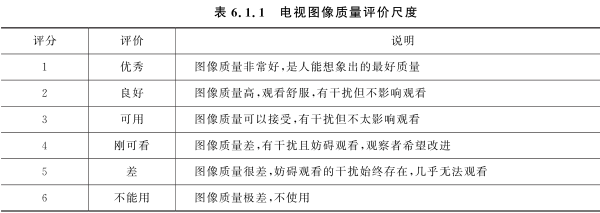
\includegraphics[scale=0.7]{37}
\end{figure}
\subsection{熵编码}
熵编码是建立在图像统计特性基础之上的一类压缩编码方法,又称统计编码。根据信源的概率分布特性,分配不同的长度的码字,降低平均码长,以提高传输速度,节省存储空间。
\subsubsection{霍夫曼编码}
根据信息论中的信源编码理论,如果编码结果使平均码长$\bar{L}$远大于图像的信息熵$H$,表明这种编码方法效率很低,占用比特数太多。

最好的编码结果是使$\bar{L}$等于或接近于$H$,这种状态的编码方法称为最佳编码,它既不丢失信息而引起图像失真,又占用最少的比特数。

熵编码的目的就是要使编码后的图像平均码长$\bar{L}$尽可能接近图像的信息熵$H$,其基本原理是根据图像灰度级出现的概率大小赋予不同长度的码字,出现概率大的灰度级赋予短码字,出现概率小的灰度级赋予长码字。这样的编码结果所获得的平均码字最短。

采用霍夫曼编码方法给每个符号分配的代码长度不是固定的,但在编码时却不需要在生成的码流中附加同步代码,原因是在解码时可按霍夫曼码本身的特性加以区分。编码时需要生成解释各种代码意义的码表,在解码时就可根据这张码表进行译码。

\begin{figure}[H]
	\centering
	\includegraphics[scale=0.6]{38}
\end{figure}
霍夫曼编码特点:

(1)霍夫曼编码构造出来的编码值不是唯一的。因为在给两个最小概率的图像的灰度值进行编码时,可以是大概率为0,小概率为1,但也可以相反;当两个灰度值的概率相等时,0,1的分配也是随机的。这就造成了编码的不唯一性,但其平均码长却是相同的,所以不影响编码效率和数据压缩性能。

(2)霍夫曼编码没有错误保护功能。如果码流中出现错误,解码时不但这个代码会译错,更糟糕的是还会导致后面的代码也会译错,这种现象称为错误传播。

(3)霍夫曼编码结果码字不等长,虽说平均码字最短,效率最高,但是码字长短不一,硬件实现很复杂,特别是译码。故又提出了双字长霍夫曼编码方法,希望通过降低效率来换取简单的硬件实验。双字长霍夫曼编码只采用两种字长的码字,对出现概率大的符号赋予短码字,对出现概率小的符号赋予长码字。短码字中留下一个码字不用,作为长码字前缀。这种方法压缩效率不如霍夫曼编码高,但其硬件实现相对简单。

(4)霍夫曼编码在实际应用中,需要与其他编码相结合,才能进一步提高数据的压缩比。例如静态图像压缩标准JPEG中,先对图像进行分块,然后进行DCT变换,量化,Z字形扫描,行程编码后,再进行霍夫曼编码。
\begin{figure}[H]
	\centering
	\includegraphics[scale=0.6]{39}
\end{figure}

\subsubsection{香农-范诺编码}
香农-范诺编码是一种常见的可变字长的编码,与霍夫曼编码相似,具体的编码步骤:

1.将信源符号按照其出现概率从大到小排列;

2.从这个概率集合中的某个位置将其分为两个子集合,并尽量使两个子集合的概率和近似相等,给前面一个子集合中只有一个元素为止;

3.重复步骤2,直到各个子集合中只有一个元素为止;

4.将每个元素所属的子集合的值依次串起来,即可得到各个元素的香农-范诺编码。

\begin{figure}[H]
	\centering
	\includegraphics[scale=0.6]{40}
\end{figure}

\subsubsection{算术编码}
从结构上分,编码有两种方式:分组编码和序列编码。

\noindent 分组编码又叫块码,是将信源消息序列分成长度为N的字符组,按组进行编码的方式;(如算术编码和游程编码)

\noindent 序列编码又叫流码,是直接为整个信源消息序列寻找编码序列的方式。等长码和变长码的编码,都是块码。

\begin{figure}[H]
	\centering
	\includegraphics[scale=0.6]{41}
\end{figure}

必须保留最后的消息符号,以作为特定的消息结束指示符,它将子区间变窄为[0.06752,0.0688)。在这个子区间内的任意数字(如0.068)都可以用来表示该消息。使用了3个十进制数字来表示这个五符号消息。就转换为每信源符号0.6个十进制数字,由信息熵的定义式,可算出信源的熵为每个信源符号0.58个十进制数字。当被编码的序列的长度增加时,得到的算术编码接近信源熵。

同样的例子,考虑霍夫曼编码过程,一个四符号信源的五符号序列或消息的霍夫曼码为0100011001.霍夫曼编码和算术编码相比较,对同样的符号序列霍夫曼码的数据量比算术码的数据量大,或者说霍夫曼编码的效率比算术编码的效率低。

\subsubsection{行程编码}
行程编码是相对简单的数据无损压缩编码技术,利用连续数据单元有相同数值这一特点对数据进行压缩。在编码时,对相同的数值只编码一次,同时计算相同数值连续重复的次数。对图像编码来说,对沿特定方向上具有相同灰度值的像素只编码一次,其延续长度称为延续的行程,简称为行程或游程。行程编码是一种无损压缩技术,这种编码方法所获得的压缩比大小主要是取决于数据本身的特点。

行程编码尤其适用于计算机生成的图像,对减少图像文件的存储空间非常有效。但行程编码对颜色丰富的自然图像压缩效果不好,因为在同一行上具有相同颜色的两虚像素很少,而连续几行都具有相同颜色值的连续行数就更少。

行程编码一般不直接应用于多灰度图像,但比较适合于二值图像的编码。行程编码与其他图像编码方法混用以获得较好的压缩效果。例如,在JPEG中,行程编码和DCT编码及霍夫曼编码一起使用,先对图像进行分块处理,然后对分块进行DCT,对量化后的频域图像数据进行Z字形扫描,再进行行程编码,最后对行程编码后的结果进行霍夫曼编码。

\subsection{预测编码}
预测编码基于图像数据的空间冗余特性,基本原理:首先根据算法模型,用原有的样本值对新样本进行预测,得到新样本的预测值;取新样本的实际数值与预测值进行比较,二者相减得到差值,最后对差值进行量化和编码。通常误差值比样本值小得多,因而可达到数据压缩地效果。

预测编码方法在图像数据压缩和语音信号数据压缩中都得到了广泛地应用。差分脉冲编码调制(DPCM)是一种具有代表性的预测编码方法。
\subsubsection{差值图像的统计特性}
由图像的统计特性可知,相邻像素之间有较强的相关性,即相邻像素的灰度值相同或相近,某像素的值可根据已知的像素来估计。一般来说,相邻量像素灰度值突变的概率小,水平方向如此,在图像的垂直方向也是如此。

经过对大量图像的差值信号统计,幅度差值愈大的差值信号出现的概率愈小,而零值或接近零值的差值信号出现的概率最大。这表现在一幅图像中都含有亮度值恒定或者变化很小的大面积区域,从而使差值信号的$80\%~90\%$落在$16~18$个量化层中。因此利用图像水平方向(或垂直方向)两个像素真实的离散幅度相减而得到它们的差值,然后对差值进行编码,传输就能达到压缩图像数据的目的。

\subsubsection{DPCM基本原理}
比价相邻的两个像素,如果两个像素之间存在差异,将差异之处的差值传送出去,若比较的像素之间没有差异,则不传送差值。

\begin{wrapfigure}{r}{5.5cm}
	\centering
	\includegraphics[width=0.23\textheight]{43}
\end{wrapfigure}
其中编码器和解码器分别完成对预测误差量化值的熵编码和解码。

设$x_N$为$t_N$时刻输入信号的亮度采样值,$\hat{x}_N$为根据$t_N$时刻以前已知的像素亮度采样值$x_1,x_2,...,x_{N-1}$对$x_N$所做的预测值,$e_N$为差值信号,也称误差信号。
$$e_N = x_N - \hat{x}_N$$
$q_N$为量化器的量化误差,$e'_N$为量化器输出信号,则有:
$$q_N = e_N - e_n'$$
接收端输出为$x'_N$,则有:
$$x'_N = \hat{x}_N + e'_N$$
那么,在接收端复原的像素值$x'_N$与发送端的原输入像素值$x_N$之间的误差为:
$$x_N - x'_N = x_N - (\hat{x}_N + e'_N) = (x_N - \hat{x}_N) - e'_N = e_N - e'_N = q_N$$
在DPCM系统中,误差的来源是发送端的量化器,而与接收端无关。
\subsubsection{DPCM预测编码方案}
若$t_N$时刻之前的已知样值与预测值之间的关系呈现某种函数的形式,该函数一般分为线性和非线性两种,所以预测编码器就有线性预测编码器和非线性预测编码器两种。

在图像数据压缩中,常见的有:

1.前值预测:即$\hat{x}_N = ax_{N-1}$

2.一维预测:即用$x_N$的同一扫描行中的前面已知的几个采样值预测$X_N$,其预测公式为:$$\hat{x}_N = \sum_{i=1}^{N-1}a_ix_i$$

3.二维预测:即用$x_N$的同一扫描行以前的几个采样值$(x_1,x_5)$,还用$x_N$的以前几行中的采样值$(x_2,x_3,x_4)$一起来预测$x_N$

4.三维预测(帧内预测):取用已知像素不但是前几行的而且还包括前几帧的来预测$x_N$,相邻帧间细节的变化很少,即相对应像素的灰度变化较小,存在极强的相关性,利用预测编码去除帧间的相关性,可以获得更大的压缩比。

\subsubsection{自适应预测编码}
DPCM系统,在输入信号为平稳的样本序列时,效果较好。但当输入数据总体平稳而局部有较大变化时,使用固定参数的预测器就会影响预测的准确性。

1.对灰度有突变的地方,会有较大的预测误差,导致重建图像的边缘模糊,分辨率降低。

2.对灰度变化缓慢的区域,其差值信号应大约为0,但因其预测值偏大而使重建图像有颗粒噪声。

为了改善图像的质量,克服上述预测编码带来的缺点,非线性预测充分考虑了图像的统计特性和个别变化,预测器的预测系数不固定,随图像的局部特性而有所变化。尽量使预测系数随预测环境而变,从而得到较为理想的输出,故称为自适应预测编码。

1977年Yamada提出一个二维DPCM的自适应预测方案,预测函数为$\hat{x}_N = K(a_1x_1 + a_4x_4)$其预测系数$a_1=0.75,a_4=0.25$,K为自适应预测参数,定义为:
$$K = \left\{\begin{matrix}
	1.0 + 0.125 &\left | e'_{N-1}\right | = e_K \\ 
	1.0 &e_1< \left | e'_{N-1}\right |< e_K \\
	1.0 - 0.125 &\left | e'_{N-1}\right | = e_1 
\end{matrix}\right.$$
式中,$e_K$为最大量化输出正电平,$e_1$为最小量化输出正电平,$e'_{N-1}$为第N-1个采样值的量化输出电平。

\subsection{变换编码}
预测编码的解压能力是有限的。DPCM只能压缩到每样值$2~4$比特。到20世纪70年代后期,研究者发现离散余弦变换(DCT)的变换矩阵来做正交变换就可以节省大量的求解特征向量的计算,因而大大简化了算法的计算复杂性。
\subsubsection{变换编码的基本原理}
变换编码就是将原来在空间域上描述的图像等信号,通过一种数学变换(如傅里叶变换,离散余弦变换,沃尔什变换等),变换到变换域中进行描述,达到改变能量分布的目的。

对于大多数图像,大量的变换系数很小,只要删除接近于0的系数,而保留包含图像主要信息的系数,达到去除相关的目的,再进行量化,编码,进一步压缩图像。在重建图像进行解码时,所损失的将是一些不重要的信息,几乎不会引起图像的失真,图像的变换编码就是利用这些来压缩图像的,因而能获得较高的压缩比。

\begin{figure}[H]
	\centering
	\includegraphics[scale=0.6]{44}
\end{figure}

变换编码首先将一幅图像进行分块处理,然后对子图像进行变换操作,解除子图像像素间的相关性,达到用少量的变换系数包含尽可能多的图像信息的目的,接下来的量化步骤是有选择地消除或粗量化带有很少信息地变换系数,因为这些系数对重建图像地质量影响很小,最后进行编码,一般采用变长码编码方法。解码是编码地相应地逆过程。
\subsubsection{变换方法的选择}
对一个给定的编码应用,如何选择变换取决于可容许的重建误差和计算要求。在理论上K-L变换是最优的正交变换,它能完全消除子项块内像素间的线性相关性。K-L变换的基向量对不同图像是不同的,且与编码对象的统计特性有关,所以一般只作为理论上的比较标准。实际图像压缩常采用DCT,它在压缩中具有广泛的应用,它是JPEG,MPEG等数据压缩标准的重要数学基础。

\begin{figure}[H]
	\centering
	\includegraphics[scale=0.6]{45}
\end{figure}

DCT压缩图像的过程如下:

\noindent1.首先将输入的图像分解为$8\times 8$或$16\times 16$的块,然后对每个子块进行二维DCT

\noindent2.将变换后得到的量化的DCT系数进行编码和传送,形成压缩后的图像格式。

DCT解压图像的过程如下:

\noindent1.对每个$8\times 8$或$16\times 16$块进行二维解码,逆量化和二维离散余弦逆变化(IDCT)

\noindent2.将逆变换的矩阵的块合成一个单一的图像。

余弦变换具有把高度相关数据能量集中的趋势,DCT后矩阵的能量集中在矩阵的左上角,右下角大多数的DCT系数值非常接近于0.压缩应该在最合理地近似原图像地情况下使用最少系数,使用系数地多少也决定了压缩比的大小。

\subsubsection{子图像尺寸的选择}
在正交变换中,需要将一帧图像划分为若干正方形的图像子块来进行。子块越小,计算量越小,计算速度快,实现简单,但均方误差较大,在同样的允许失真度下,压缩比小。但子块太大,压缩量增大,使得计算复杂度也显著加大。

一般情况下,压缩量和计算复杂度都随子图像尺寸的增加而增加。子图像的长和宽都是2的整数次幂,常用的子图像尺寸为$8\times 8$和$16\times 16$
\subsubsection{变换系数的选择}
子图像经过变换后,保留变换后的变换系数直接影响信号的恢复质量,变换系数的选择原则是保留变换系数中幅值较大的元素,而将大多数幅值较小或某些特定区域的变换系数作零处理。

系数选择通常有区域编码和阈值编码

\noindent1.区域编码:对设定形状的区域内的变换系数进行量化编码,区域外的系数被舍去。保留区域的左上部,即低频分量都集中在此部分,但是高频分量完全丢失,反应在重建图像上就是轮廓及细节模糊。

\noindent2.阈值编码:对所有子图像采用一个固定的模板,自适应地为各个子图像设置不同地模板。多数低频成分被编码输出,而且少数超过阈值地高频成分也被保留下来进行编码输出。

选取阈值的方法:1.对所有子图像采用1个全局阈值。2.对各个子图像分别用不同地阈值。3.根据子图像中各系数地位置选取阈值。

\subsubsection{静止图像压缩编码标准JPEG}
JPEG(Joint Photographic Experts Group)是联合图像专家小组的缩写,所谓联合是指国际标准化组织ISO和国际电报电话咨询委员会(CCITT)的联合。联合图像专家小组于1986年成立,任务是开发研制连续色调,多级灰度,静止图像的数字图像压缩编码标准:

1.必须将图像质量控制在可视保真度高的范围内,同时编码器可被参数化,允许用户设置压缩或质量水平。

2.压缩标准可以应用于任何一类连续色调数字图像,并不应受到维数,颜色,画面尺寸,内容,影调的限制。

3.压缩标准必须从完全无损到有损范围内可选,以适应不同的存储。

JPEG标准是为连续色调图像的压缩提供的公共标准,连续色调图像并不局限于单色调图像。该标准可适用于各种多媒体存储和通信应用所使用的灰度图像,摄影图像及静止视频压缩文件。具有高压缩比的特征。

\textbf{原理}

$8\times 8$的图像经过DCT后,其低频分量都集中在左上角,高频分量分布在右下角。并使用量化操作将高频分量去除。所谓的量化操作,就是将某一个值除以量化表中对应的值。由于量化表左上角的值较小,右下角的值较大,这样就起到了保留低频分量,抑制高频分量的目的。

\textbf{编码流程}

\begin{figure}[H]
	\centering
	\includegraphics[scale=0.6]{46}
\end{figure}

(1)颜色空间转换,数据分块及采样

在彩色图像中,人眼对色彩的变化不如对亮度的变化敏感,一般先将图像从RGB空间转换到$YC_bC_r$空间。在颜色空间转换完成之后,将每个分量图像分割成不重叠的$8\times 8$像素块,每个$8\times 8$像素块称为一个数据单元(DU)。在对图像采样时,可以采用不同的采样频率。由于亮度比色彩更重要,因此对Y分量的采样频率要高于对$C_b,C_r$的采样频率,这样有利于节省存储空间。常用的采样格式有$4:2:2$和$4:1:1$

(2)$8\times 8$子块DCT

为了提高压缩效率,考虑到局部子块中图像的相关性强的事实,通常采用的方法是,将图像分为$8\times 8$的子块,对每个子块独立地进行DCT

DCT的公式:
$$F(u,v) = \frac{C(u)C(v)}{4}[\sum_{i=0}^{7}\sum_{j=0}^{7}f(i,j)cos\frac{(2i+1)u\pi}{16}cos\frac{(2j+1)v\pi}{16}](u,v=0,1,...,7)$$
其逆变换公式为:
$$f(i,j) = \frac{1}{4}[\sum_{i=0}^{7}\sum_{j=0}^{7}C(u)C(v)F(u,v)cos\frac{(2i+1)u\pi}{16}cos\frac{(2j+1)v\pi}{16}](i,j=0,1,...,7)$$
其中,
$$C(u),C(v) = \left\{\begin{matrix}
	\frac{1}{\sqrt{2}}, &\text{当}u=v=0 \\ 
	1, &\text{其他}
\end{matrix}\right.$$

随着u和v的增加,相应系数分别代表逐步增加的水平空间频率和垂直空间分量的大小。右上角的系数表示水平方向频率最高,垂直方向频率最低的分量大小;右下角的系数表示水平方向频率最低,垂直方向频率最高的分量大小。右下角表示水平方向频率和垂直方向频率都最高的分量大小。

(3)系数矩阵量化

在量化过程中,应根据人眼的视觉特性,对于可见度阈值大的频率分量允许有较大的量化误差,使用较大的量化步长(量化间隔)进行粗量化;而对可见度阈值小的频率分量应保证有较小的量化误差,使用较小的量化步长进行细量化。

量化间隔的大小决定了量化的精度。按照人眼对低频分量比较敏感,对高频分量不太敏感的特性,需要对不同的变换系数设置不同的量化步长。

\begin{figure}[H]
	\centering
	\includegraphics[scale=0.6]{47}
\end{figure}

这两个量化表中量化步长值是通过大量实验并根据主观评价效果确定的,其值随DCT系数的位置而改变,同一像素的亮度量化表和色度量化表不同。

(4)Z字形扫描

经过DCT后,低频分量集中在左上角,其中$F(0,0)$代表DC系数,即$8\times 8$子块的平均值,要对它进行单独编码。由于两个相邻的$8\times 8$子块的DC系数相差很小,所以对它们采用差分编码(DPCM)可以提高压缩比。$8\times 8$的其他63个元素是AC系数,采用行程编码。
\begin{figure}[H]
	\centering
	\includegraphics[scale=0.6]{48}
\end{figure}

(5)熵编码输出

Z字形扫描之后对一维序列进行后续的编码,如Huffman编码,游程编码等。

接收短解码器经熵编码,逆量化后得到带有一定量化失真的变换系数$F'(u,v)$,再经DCT逆变换就得到重建图像块的样本值$f'(x,y)$。与原始图像块相比较,两者数据大小非常接近,其误差主要是由量化造成的。只要量化器设计得好,失真可限制在允许得范围,故为限失真编码。

\section{图像分割}
\subsection{概述}
\subsubsection{图像分割的概念}
在对图像的研究和应用中,人们往往仅对某幅图像中的某些部分感兴趣,这些部分常称为目标或前景,它们一般对应图像中特定的,具有独特性质的区域。为了辨识和分析目标,需要将这些有关区域分离提取出来,在此基础上才有可能对目标进一步利用,如进行特征提取和测量。

图像分割按照图像的某种特性(如灰度级),把图像分割成不同的区域,或把不同的目标分割开,或把图像分成互不重叠的各具特性的区域并提取感兴趣目标的技术和过程。

\subsubsection{图像分割的方法}
在已提出的算法中,较为经典的有阈值分割法,边缘检测法和区域分割法。近十年有一些特殊理论如数学形态学,小波分析,模糊数学。

\begin{figure}[H]
	\centering
	\includegraphics[scale=0.6]{49}
\end{figure}

\subsection{阈值分割法}
寻找适当的灰度阈值。通过人眼的观察,对已知某些特征的图像,只要试验不同的阈值,然后看是否满足已知特征,但这种方法的问题是使用范围窄,使用前必须事先知道图像的某些特征,如平均灰度等,而且分割后图像质量的好坏受主观局限性很大。

使用一个或几个阈值将图像的灰度级分为几个部分,认为属于同一个部分的像素是同一个物体。该方法的最大特点是计算简单。

\subsubsection{灰度阈值法}
若图像中目标和背景具有不同的灰度集合,即目标灰度集合与背景灰度集合,且两个灰度集合可用一个灰度级阈值T进行分割。在目标物体与背景有较强的对比度的图像中,此方法应用特别有效。

设图像$f(x,y)$的灰度级范围是$[0,L-1]$,那么在0和$L-1$之间选择一个合适的灰度值T作为阈值,就可以定义阈值化后的二值图像。

1.阈值化后的图像定义为:
$$g(x,y) = \left\{\begin{matrix}
	1 &f(x,y) \geqslant T\\ 
	0 &f(x,y) < T
\end{matrix}\right.$$

2.阈值化后的图像定义为:
$$g(x,y) = \left\{\begin{matrix}
	1 &f(x,y) \leqslant T\\ 
	0 &f(x,y) > T
\end{matrix}\right.$$
这种灰度阈值分割也叫图像二值化处理,它的目的就是求一个阈值T,并用T将图像$f(x,y)$分成目标和背景两个区域。

在实际处理图像时,由于目标和背景并不一定单纯地分布在两个灰度范围内,故要对基本阈值进行修正。
$$g(x,y) = \left\{\begin{matrix}
	1 &T_1 \leqslant f(x,y) \leqslant T_2 \\ 
	0 &\text{其他}
\end{matrix}\right.$$
或
$$g(x,y) = \left\{\begin{matrix}
	0 &T_1 \leqslant f(x,y) \leqslant T_2 \\ 
	1 &\text{其他}
\end{matrix}\right.$$

阈值地选取方法很多,通常根据先验知识确定阈值,或者利用灰度直方图特征和统计判决方法确定灰度分割阈值。

在利用直方图取阈值方法来分割灰度图像时,图像有一定的假设。假设图像由具有单峰灰度分布的目标和背景组成,处于目标和背景内部相邻像素间的灰度值是高度相关的,但处于目标和背景交界的两边的像素在灰度值上有很大的差别,它的灰度直方图基本可看作由分别对应目标和背景的两个单峰直方图混合构成。如果这两个分布大小接近且均值相距足够远,而且两部分的均方差也足够小,则直方图有较明显的双峰。

若灰度图像的直方图灰度级范围为$i=0,1,...,L-1$当灰度级为$k$时的像素数为$n_k$则一幅图像的总像素N为:
$$ N = \sum_{i=0}^{L-1}n_i = n_0 + n_1 + ... + n_{L-1}$$
灰度级i出现的概率为:
$$p_i = \frac{n_i}{N} = \frac{n_i}{n_0 + n_1 + n_2 + ... + n_{L-1}}$$
\begin{wrapfigure}{r}{5.5cm}
	\centering
	\includegraphics[width=0.23\textheight]{50}
\end{wrapfigure}

背景和对象在图像的灰度直方图上各自形成一个波峰,由于每两个波峰间形成一个低谷,因而选择双峰间低谷处所对应的灰度值为阈值,可将两个区域分离。这种通过选取直方图阈值来分割目标和背景的方法称为直方图阈值双峰法。

用直方图双峰法进行图像分割的算法实现:

1.对图像进行灰度变换,得到其灰度图像。

2.做出灰度图像的直方图。

3.若只出现背景和目标两区域部分所对应的直方图呈双峰且有明显的谷底,则可将谷底点所对应的灰度值t作为阈值T。

4.根据阈值T,进行图像扫描,凡灰度级大于T的,颜色设置为255;凡灰度级小于T的,颜色设为0。

\subsubsection{最大类间方差法}
当图像中的目标部分和背景之间的灰度级较小,灰度直方图的双峰特性不明显,可采用最大方差阈值法。

假设某个图像的灰度直方图包含两类区域,T为分离两类区域的阈值。L为图像的灰度级数,$f_i$为灰度级i的所有像素个数。经统计可得,被T分离后的区域1,区域2占整个图像的面积以及区域1,区域2,整幅图像的平均灰度如下:

区域1的面积比$$\theta_1 = \sum_{i=0}^{T}\frac{n_i}{n}$$

区域2的面积比$$\theta_2 = \sum_{i=T+1}^{L-1}\frac{n_i}{n}$$

整幅图像的平均灰度$$\mu = \sum_{i=0}^{L-1}f_i\times \frac{n_i}{n}$$

区域1的平均灰度$$\mu_1 = \frac{1}{\theta_1}\sum_{i=0}^{T}f_i\times \frac{n_i}{n}$$

区域2的平均灰度$$\mu_2 = \frac{1}{\theta_2}\sum_{i=T+1}^{L-1}f_i\times \frac{n_i}{n}$$

整幅图像的平均灰度级与区域1,区域2的平均灰度级之间的关系为:
$$\mu = \mu_1\theta_1 + \mu_2\theta_2$$

区域间的方差可表示为:$$\sigma_B^2 = \theta_1(\mu_1-\mu)^2 + \theta_2(\mu_2-\mu)^2$$
式中,$\sigma_B^2$表示图像被阈值T分割后两个区域之间的方差。被分割的两个区域之间方差$\sigma_B^2$达到最大时,被认为是两个区域的最佳分离状态。

\begin{wrapfigure}{r}{5.5cm}
	\centering
	\includegraphics[width=0.23\textheight]{51}
\end{wrapfigure}

最大类间方差的具体算法如下:

1.将RGB图像转换为灰度图像

2.求出图像中的所有像素的分布概率$p_1,p_2,...,p_255$

3.给定一个初始阈值$T_h = T_{h0}$,将图像分为$C_1$和$C_2$两类

4.根据公式$\sigma_i^2 = \sum_{(x,y)\in C_i}(f(x,y) - \mu_i)^2$和$\mu_i = \frac{1}{N_{C_i}}\sum_{(x,y)\in C_i}f(x,y)(i=1,2)$分别计算两类的方差$\sigma_1^2$和$\sigma_2^2$以及图像的整体平均灰度值$\mu$
$$\mu = \frac{1}{N_{image}}\sum_{i=1}^{m}\sum_{j=1}^{n}f(i,j)$$
式中,$N_{image}$为图像的总体像数。

5.计算两类问题发生的概率$p_1$和$p_2$
$$p_1 = \sum_{i=1}^{T_h}p_i, \qquad p_2 = 1-p_1$$

6.计算类间方差$\sigma_m^2$和类内方差$\sigma_n^2$
$$\sigma_m^2 = p_1\cdot (\mu_1 - \mu)^2 + p_2\cdot (\mu_2 - \mu)^2$$
$$\sigma_n^2 = p_1\cdot \sigma_1^2 + p_2\cdot \sigma_2^2$$

7.选择最佳阈值$T_h = T_h^*$,使得图像按照该阈值分为$C_1$和$C_2$两类后,满足$$\eta = max\{ \frac{\sigma_m^2}{\sigma_n^2}\}$$

\subsubsection{迭代阈值法}
迭代阈值法是阈值法图像分割中较有效的方法,通过迭代的方法来求出分割的最佳阈值,具有一定的自适应性。

1.设定参数$T_0$,并选择一个初始的估计阈值$T_1$.

2.用阈值$T_1$分割图像,将图像分成两个部分:$G_1$是由灰度值大于$T_1$的像素组成的,$G_2$是由灰度值小于或等于$T_1$的像素组成的。

3.计算$G_1$和$G_2$中所有的像素的平均灰度值$\mu_1$和$\mu_2$以及新的阈值$T_2  = (\mu_1 + \mu_2)/2$

4.如果$|T_2 - T_1|<T_0$,则推出$T_2$即为最优阈值;否则,将$T_2$幅值给$T_1$并重复步骤$1~4$,直到获得最优阈值。

\section{图像配准}
图像配准是一种重要的数字图像处理应用,它用于对齐同一场景的两幅或多幅图像。在图像配准中,我们有一幅输入图像和一幅参考图像,目的是对输入图像做几何变换,使输出图像与参考图像对齐(配准)。

图像配准的图像包括对齐两幅或多幅几乎同一时间但用不同成像系统,图像也可以是使用相同的设备在不同的时间拍摄的。无论属于哪种情况,组合这些图像或对这些图像进行定量分析并比较,都要求对几何失真进行补偿,其中几何失真由视角,距离,方向,传感器分辨率,物体位置的移动和其他因素导致。

我们使用约束点(控制点)解决几何失真补偿问题。这些点是其精确位置在输入图像和参照图像中已知的对应点。选取约束点的方法有多种,既可以交互地选择,也可以用自动检测算法进行选择。某些成像系统地成像传感器中嵌入了物理赝像(如小金属物),它们会在系统获取的所有图像上直接产生一组已知点(网状标记或基准点)。这些点可用于指导建立约束点。

假设在输入图像和参考图像中都有4个约束点。求出我们变换输入图像中的所有像素的工具中的系数后,我们令$(v,w)$表示输入图像中每个像素的坐标,令$(x,y)$代表输出图像中对应像素的坐标。我们遍历输入图像中的所有$(v,w)$来产生输出图像(即配准图像)中的对应$(x,y)$。如果约束点选择得正确,那么新图像就能在双线性近似模型得精度范围内与参考图像配准。

在4个约束点不足以得到令人满足得配准得情况下,常用得一种方法是选择大量得约束点,然后将一系列4约束点形成得四边形当作子图像进行处理。子图像采用上述处理,四边形内部得所有像素则使用由该四边形得约束点求出的系数进行变换。然后,移到另一组4约束点并重复上述过程,直到所有四边形区域均被处理为止。也可以采用比四边形更加复杂的区域。


































































































































































































































































































































































































































































































































































































































\end{document}